 %\documentclass[preprint,12pt]{elsarticle}

%% Use the options 1p,twocolumn; 3p; 3p,twocolumn; 5p; or 5p,twocolumn
%% for a journal layout:
%%  \documentclass[final,1p,times]{elsarticle}
%% \documentclass[final,1p,times,twocolumn]{elsarticle}
%% \documentclass[final,3p,times]{elsarticle}
%% \documentclass[final,3p,times,twocolumn]{elsarticle}
%\documentclass[final,5p,times]{elsarticle}
\documentclass[final,5p,times,twocolumn]{elsarticle}

\newcommand{\note}[2][inline]{\todo[color=red!30,#1]{\small\sf #2}}

%% if you use PostScript figures in your article
%% use the graphics package for simple commands
%% \usepackage{graphics}
%% or use the graphicx package for more complicated commands
%% \usepackage{graphicx}
%% or use the epsfig package if you prefer to use the old commands
%% \usepackage{epsfig}

%% The amssymb package provides various useful mathematical symbols
\usepackage{rotating,todonotes, xspace}
\usepackage{amssymb}
\usepackage[section]{placeins}
\usepackage{makeidx}  % allows for indexgeneration
\usepackage{algorithm}
\usepackage{algpseudocode}
\usepackage{graphicx}
\usepackage{float}
\usepackage{subcaption}
\captionsetup{compatibility=false}
\usepackage{wrapfig}
\usepackage{array}
\usepackage{multicol}
\usepackage{hyperref}
\usepackage{enumitem}

% The amsthm package provides extended theorem environments
%% \usepackage{amsthm}


\journal{Future Generation of Computer Systems}
\newcommand{\rev}[1]{\color{blue} #1\color{black}}

\begin{document}

\begin{frontmatter}

%Should change the tilte to something better
\title{Using Imbalance Metrics to Optimize Task Clustering in Scientific Workflow Executions}


\author[isi]{Weiwei Chen\corref{cor1}}
\ead{weiweich@acm.org}

\author[isi]{Rafael Ferreira da Silva}
\ead{rafsilva@isi.edu}

\author[isi]{Ewa Deelman}
\ead{deelman@isi.edu}

\author[man]{Rizos Sakellariou}
\ead{rizos@cs.man.ac.uk}

\cortext[cor1]{Corresponding address: USC Information Sciences Institute, 4676 Admiralty Way Ste 1001, Marina del Rey, CA, USA, 90292, Tel: +1 310 448-8408}


\address[isi]{University of Southern California, Information Sciences Institute, Marina del Rey, CA, USA}
\address[man]{University of Manchester, School of Computer Science, Manchester, U.K.}


\begin{abstract}
Scientific workflows can be composed of many fine computational granularity tasks. The runtime of these tasks may be shorter than the duration of system overheads, for example, when using multiple resources of a cloud infrastructure. Task clustering is a runtime optimization technique that merges multiple short running tasks into a single job such that the scheduling overhead is reduced and the overall runtime performance is improved. However, existing task clustering strategies only provide a coarse-grained approach that relies on an over-simplified workflow model. In this work, we examine the reasons that cause Runtime Imbalance and Dependency Imbalance in task clustering. Then, we propose quantitative metrics to evaluate the severity of the two imbalance problems. Furthermore, we propose a series of task balancing methods (horizontal and vertical) to address the load balance problem when performing task clustering for five widely used scientific workflows. Finally, we analyze the relationship between these metric values and the performance of proposed task balancing methods. A trace-based simulation shows that our methods can significantly decrease the runtime of workflow applications when compared to a baseline execution. We also compare the performance of our methods with two algorithms described in the literature.

\end{abstract}

\begin{keyword}
Scientific workflows \sep Performance analysis \sep Scheduling \sep Workflow simulation \sep Task clustering \sep Load balancing
\end{keyword}

\end{frontmatter}

\section{Introduction}
\label{intro}
Many computational scientists develop and use large-scale, loosely-coupled applications that are often structured as scientific workflows. Although the majority of the tasks within these applications are often relatively short running (from a few seconds to a few minutes), in aggregate they represent a significant amount of computation and data~\cite{daSilva:2013:TFO:2534248.2534254,Juve2013}. When executing these applications in a multi-machine{, }distributed environment, such as the Grid or the Cloud, significant system overheads may exist and may slowdown the application {execution}~\cite{Chen2011}. To reduce the impact of such overheads, task clustering techniques~\cite{Muthuvelu:2005:DJG:1082290.1082297,4493929,Muthuvelu2010,Muthuvelu2013170,keat-2006,ang-2009,Liu2009,Singh:2008:WTC:1341811.1341822,Ferreira-granularity-2013} have been developed to group \emph{fine-grained} tasks into \emph{coarse-grained} tasks so that the number of computational activities is reduced and {so that }their computational granularity is increased{.  This reduced }the (mostly scheduling related) system overheads.
However, there are several challenges that have not yet been addressed.

A scientific workflow is typically represented as a directed acyclic graph (DAG). {The nodes represent computations and the edges describe data and control dependencies between them. }Tasks within a level (or depth within a workflow DAG) may have different runtimes. {Proposed task clustering techniques that merge  }tasks within a level without considering the runtime variance may cause load imbalance, i.e., some clustered jobs may be composed of short running tasks while others of long running tasks. This imbalance delays the release of tasks from the next level of the workflow, penalizing the workflow execution with an overhead produced by the use of inappropriate task clustering strategies~\cite{Chen2013}.
A common technique to handle load imbalance is overdecomposition~\cite{Lifflander}.
This method decomposes computational work into \emph{medium-grained} balanced tasks. Each task is coarse-grained enough to enable efficient execution and reduce scheduling overheads, while being fine-grained enough to expose significantly higher application-level parallelism than what is offered by the hardware. 

Data dependencies between workflow tasks play an important role when clustering tasks within a level. A data dependency means that there is a data transfer between two tasks (output data for one and input data for the other). Grouping tasks without considering these dependencies may lead to data locality problems{, }where output data produced by parent tasks are poorly distributed. As a result, data transfer times and failure probabilities increase.
Therefore, we claim that data dependencies of subsequent tasks should be considered.

We generalize these two challenges (Runtime Imbalance and Dependency Imbalance) to the general task clustering load balance problem. We introduce a series of balancing methods to address these challenges. However, there is a tradeoff between runtime and data dependency balancing. For instance, balancing runtime may aggravate the Dependency Imbalance problem, and vice versa. Therefore, we propose a series of quantitative metrics that reflect the internal structure (in terms of task runtimes and dependencies) of the workflow and use them as a criterion to select and balance {the } solutions.

In particular, we provide a novel approach to capture {the imbalance } metrics. Traditionally, there are two approaches to improve the performance of task clustering. The first one is a top-down approach \cite{6217508} that represents the clustering problem as a global optimization problem and aims to minimize the overall workflow execution time. However, the complexity of solving such an optimization problem does not scale well since most solutions are based on genetic algorithms. The second one is a bottom-up approach~\cite{Muthuvelu:2005:DJG:1082290.1082297,Liu2009} that only examines free tasks to be merged and optimizes the clustering results locally. In contrast, our work extends these approaches to consider the neighboring tasks including siblings, parents, and children{, } because such a family of tasks has strong connections between them. 

The quantitative metrics and balancing methods were introduced and evaluated in~\cite{6683907} on {five }workflows. In this {paper}, we extend this previous work by studying:

\begin{itemize}[noitemsep,nolistsep]
	\item the performance gain of using our balancing methods over a baseline execution on a larger set of workflows;
	\item the performance gain over two additional task clustering methods described in the literature~\cite{ang-2009,Liu2009};
	\item the performance impact of the variation of the average data size and number of resources;
	\item the performance impact of combining our balancing methods with vertical clustering.
\end{itemize}

The rest of {the paper } is organized as follows. Section~\ref{sec:related-work} gives an overview of the related work. Section~\ref{sec:model} presents our workflow and execution environment models. Section~\ref{sec:imbalance} details our heuristics and algorithms for balancing. Section~\ref{sec:experiments} reports experiments and results, and the {paper } closes with a discussion and conclusions.

% Section
\section{Related Work}
\label{sec:related-work}

{System }overhead analysis~\cite{Ostberg2011, Prodan2008} is a topic of great interest in the {distributed computing } community. Stratan et al.~\cite{Stratan2008} evaluate in a real-world environment Grid workflow engines including DAGMan/Condor and Karajan/Globus. Their methodology focuses on five system characteristics: overhead, raw performance, stability, scalability, and reliability. They {point } out that {resource consumption in head nodes }should not be {ignored } and {that } the main bottleneck in a busy system is often the head node. Prodan et al.~\cite{Prodan2008} offered a complete Grid workflow overhead classification and a systematic measurement of overheads. In Chen et al.~\cite{Chen2011}, we extended~\cite{Prodan2008} by providing a measurement of major overheads imposed by workflow management systems and execution environments and analyzed how existing optimization techniques improve {the workflow }runtime by reducing or overlapping overheads. The prevalent existence of system overheads is an important reason why task clustering provides significant performance improvement for workflow-based applications. In this chapter, we aim to further improve the performance of task clustering under imbalanced load. 

The low performance of \emph{fine-grained} tasks is a common problem in widely distributed platforms where the scheduling overhead and queuing times at resources are high, such as Grid and Cloud systems. Several works have addressed the control of task granularity of bags of tasks. For instance, Muthuvelu et al.~\cite{Muthuvelu:2005:DJG:1082290.1082297} proposed a clustering algorithm that groups bags of tasks based on their runtime---tasks are grouped up to the resource capacity. Later, they extended their work~\cite{4493929} to determine task granularity based on task file size, CPU time, and resource constraints. Recently, they proposed an online scheduling algorithm~\cite{Muthuvelu2010,Muthuvelu2013170} that groups tasks based on resource network utilization, user's budget, and application deadline. Ng et al.~\cite{keat-2006} and Ang et al.~\cite{ang-2009} introduced bandwidth in the scheduling framework to enhance the performance of task scheduling. Longer tasks are assigned to resources with better bandwidth. Liu and Liao~\cite{Liu2009} proposed an adaptive fine-grained job scheduling algorithm to group fine-grained tasks according to processing capacity and bandwidth of the current available resources. Although these techniques significantly reduce the impact of scheduling and queuing time overhead, they {do } not consider data dependencies.

Task granularity control has also been addressed in scientific workflows. For instance, Singh et al.~\cite{Singh:2008:WTC:1341811.1341822} proposed level- and label-based clustering. In level-based clustering, tasks at the same level {of the workflow }can be clustered together. The number of clusters or tasks per cluster are specified by the user. In the label-based clustering {method}, the user labels tasks that should be clustered together. Although their work considers data dependencies between workflow levels, it is done manually by the users, which is prone to errors {and it is not scalable}. Recently, Ferreira da Silva et al.~\cite{Ferreira-granularity-2013,FerreiradaSilva-CCPE-2014} proposed task grouping and ungrouping algorithms to control workflow task granularity in a non-clairvoyant and online context, where none or few characteristics about the application or resources are known in advance. Their work significantly reduced scheduling and queuing time overheads, but did not consider data dependencies.

A plethora of balanced scheduling algorithms have been developed in the networking and operating system domains. Many of these schedulers have been extended to the hierarchical setting. Lifflander et al.~\cite{Lifflander} proposed to use work stealing and a hierarchical persistence-based rebalancing algorithm to address the imbalance problem in scheduling. Zheng et al.~\cite{Zheng} presented an automatic hierarchical load balancing method that overcomes the scalability challenges of centralized schemes and poor solutions of traditional distributed schemes. There are other scheduling algorithms~\cite{rizos2008} that indirectly achieve load balancing of workflows through makespan minimization. However, the benefit that can be achieved through traditional scheduling optimization is limited by its complexity. The performance gain of task clustering is primarily determined by the ratio between system overheads and task runtime, which is more substantial in modern distributed systems such as Clouds and Grids. 

Workflow patterns~\cite{Yu2005, Juve2013, Liu2008} are used to capture and abstract the common structure within a workflow and they give insights on designing new workflows and optimization methods. Yu and Buyya~\cite{Yu2005} proposed a taxonomy that characterizes and classifies various approaches for building and executing workflows on Grids. They also provided a survey of several representative Grid workflow systems developed by various projects world-wide to demonstrate the comprehensiveness of the taxonomy. Juve et al.~\cite{Juve2013} provided a characterization of workflow from six scientific applications and obtained task-level performance metrics (I/O, CPU, and memory consumption). They also presented an execution profile for each workflow running at a typical scale and managed by the Pegasus workflow management system~\cite{Deelman2004, Deelman:2005:PFM:1239649.1239653, deelman2014pegasus}. Liu et al.~\cite{Liu2008} proposed a novel pattern based time-series forecasting strategy which utilizes a periodical sampling plan to build representative duration series. We illustrate the relationship between the workflow patterns (asymmetric or symmetric workflows) and the performance of our balancing algorithms. 

Some work in the literature has further attempted to define and model workflow characteristics with quantitative metrics. In~\cite{Ali2004}, the authors proposed a robustness metric for resource allocation in parallel and distributed systems and accordingly customized the definition of robustness. Tolosana et al.~\cite{Tolosana2011} defined a metric called Quality of Resilience to assess how resilient workflow enactment is likely to be in the presence of failures. Ma et al. ~\cite{Ma:2014:GDB:2560969.2561388} proposed a graph distance based metric for measuring the similarity between data oriented workflows with variable time constraints, where a formal structure called time dependency graph (TDG) is proposed and further used as representation model of workflows. Similarity comparison between two workflows can be reduced to computing the similarity between TDGs. In this work, we develop quantitative metrics to measure the severity of the imbalance problem in task clustering and then use the results to guide the selection of different task clustering methods.



\section{Model and Design}
\label{sec:model}


A workflow is modeled as a directed acyclic graph (DAG), where each node in the DAG often represents a workflow task ($t$), and the edges represent dependencies between the tasks that constrain the order in which tasks are executed. Dependencies typically represent data-flow dependencies in the application, where the output files produced by one task are used as inputs of another task. Each task is a computational program and a set of parameters that need to be executed. 
%Figure~\ref{fig:model_odag} (left) shows an illustration of a DAG composed of four tasks. 
This model fits several workflow management systems such as Pegasus~\cite{Deelman:2005:PFM:1239649.1239653}, Askalon~\cite{Fahringer:2005:ATS:1064323.1064331}, Taverna~\cite{Oinn:2006:TLC:1148437.1148448} and {Galaxy~\cite{22559942}. }In this paper, we assume {that }there is only one execution site with multiple compute resources, such as virtual machines on the clouds. 


Figure~\ref{fig:model_system} shows a typical workflow execution environment. The {\textbf{submit host} }prepares a workflow for execution (clustering, mapping, etc.), and worker nodes, at an execution site, execute jobs individually. The main components are introduced below:

\begin{figure}[!htb]
\centering
  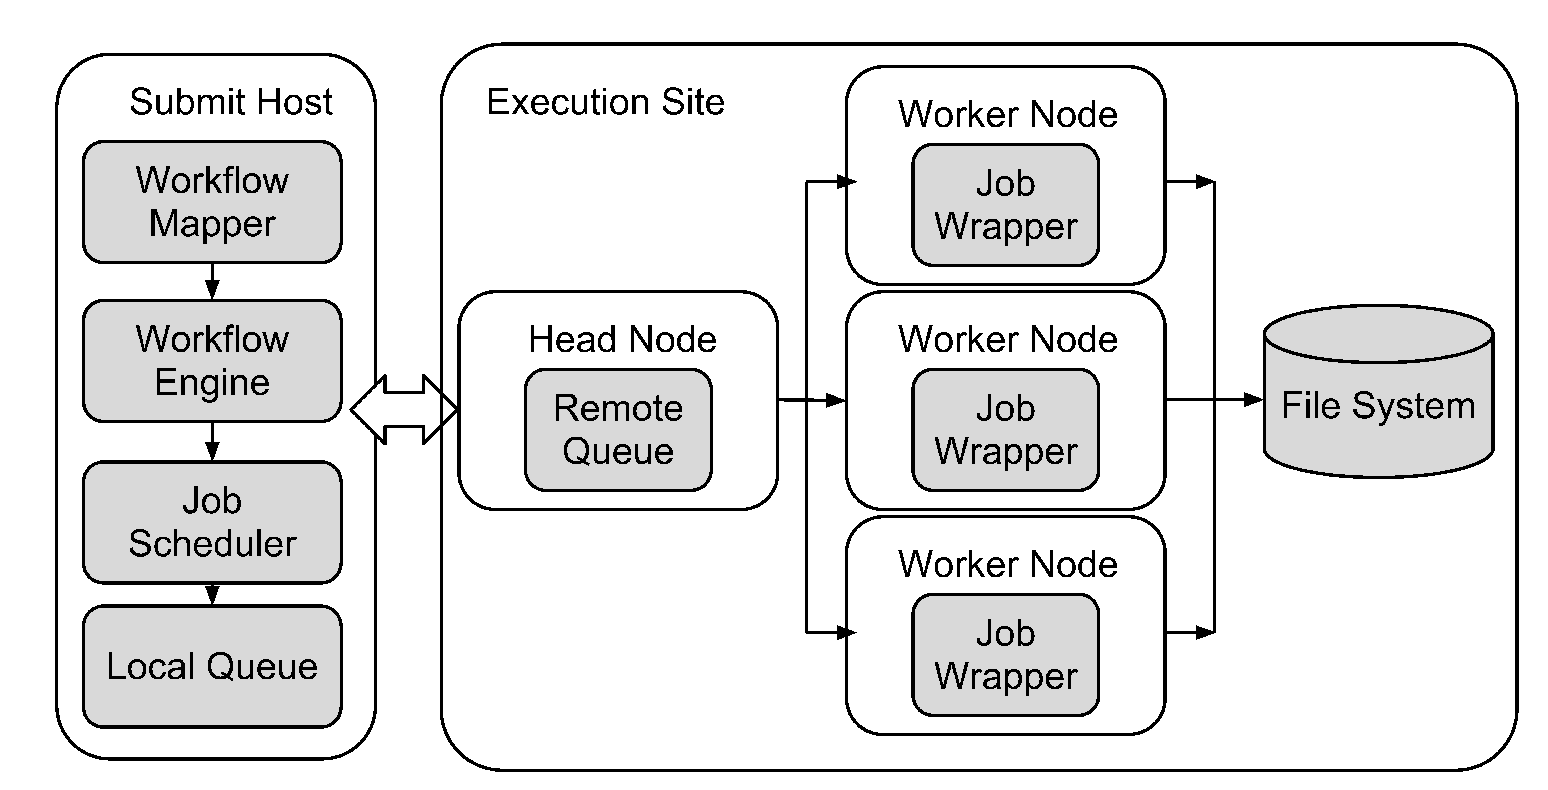
\includegraphics[width=0.95\linewidth]{figure1.eps}
  \caption{A workflow system model.}
  \label{fig:model_system}
\end{figure}

\paragraph{Workflow Mapper} Generates an executable workflow based on an abstract workflow~\cite{Deelman2004} provided by the user or workflow composition system. It also restructures the workflow to optimize performance and adds tasks for data management and provenance information generation. {The Workflow Mapper also merges }small tasks together into a job such that system overheads are reduced (\textbf{task clustering}). A job is a single execution unit in the workflow execution systems and is composed of one or more tasks. 


\paragraph{Workflow Engine} Executes jobs defined by the workflow in order of their dependencies. Only jobs that have all their parent jobs completed are submitted to the Job Scheduler. The elapsed time from when a job is released (all of its parents have completed successfully) to when it is submitted to the job scheduler is denoted as the workflow engine delay. %The workflow engine delay is usually configured by users to assure that the entire workflow scheduling and execution system is not overloaded. 

\paragraph{Job Scheduler and Local Queue} Manage individual workflow jobs and supervise their execution on local and remote resources. {The scheduler relies on the resources (compute, storage, and network) defined in the executable workflow to perform computations. }The elapsed time from when a task is submitted to the job scheduler to when it starts its execution in a worker node is denoted as the queue delay. It reflects both the efficiency of the job scheduler and resource availability. 

\paragraph{Job Wrapper} Extracts tasks from clustered jobs and executes them at the worker nodes. The clustering delay is the  elapsed time of the extraction process.

\begin{figure}[!htb]
	\centering
	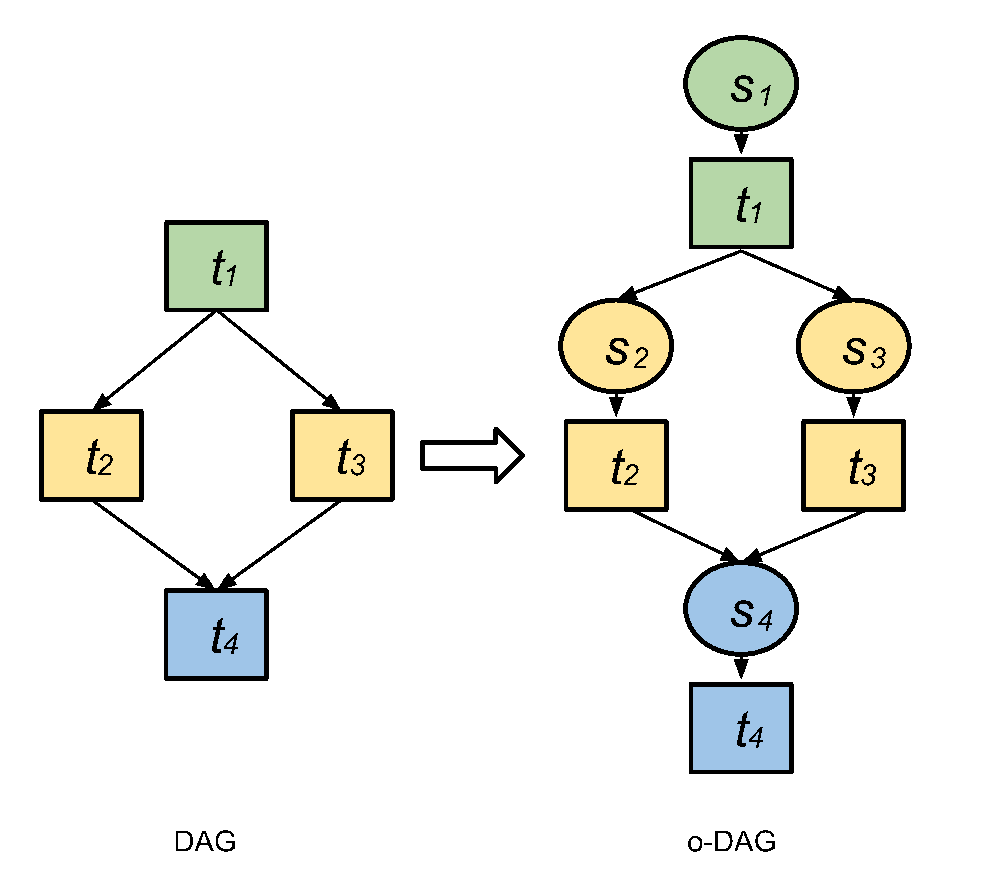
\includegraphics[width=0.7\linewidth]{figure2.eps}
	\captionof{figure}{Extending DAG to o-DAG (\emph{s} denotes a system overhead).}
	\label{fig:model_odag}
\end{figure}

We extend the DAG model to be overhead aware (o-DAG). System overheads play an important role in workflow execution and constitute a major part of the overall runtime when tasks are poorly clustered~\cite{Chen2011}. Figure~\ref{fig:model_odag} shows how we augment a DAG to be an o-DAG with the capability to represent system overheads ($s$) such as workflow engine and queue delays. In addition, system overheads also include data transfer {delays }caused by staging-in and staging-out data. This classification of system overheads is based on our prior study on workflow analysis~\cite{Chen2011}. 

With an o-DAG model, we can explicitly express the process of task clustering. In this paper, we address {horizontal and vertical task clustering}. \textbf{Horizontal Clustering} (HC) merges multiple tasks that are at the same horizontal level of the workflow, in which the horizontal level of a task is defined as the longest distance from the entry task{(s) }of the DAG to this task {(an entry task has no parents)}. \textbf{Vertical Clustering} (VC) merges tasks within a pipeline of the workflow. Tasks {in }the same pipeline share a single-parent-single-child relationship, which means a task $t_a$ is the unique parent of a task $t_b$, which is the unique child of $t_a$. 

Figure~\ref{fig:model_hc} shows a simple example of how to perform HC, in which two tasks $t_2$ and $t_3$, without a data dependency between them, are merged into a clustered job $j_1$. A job $j$ is a single execution unit composed by one or multiple task(s). Job wrappers are commonly used to execute clustered jobs, but they add an overhead denoted by the clustering delay $c$. The clustering delay measures the difference between the sum of the actual task runtimes and the job runtime seen by the job scheduler. 
After horizontal clustering, $t_2$ and $t_3$ in $j_1$ can be executed in sequence or in parallel, if parallelism {on }one compute node is supported. In this paper, we consider sequential executions only. Given a single resource, the overall runtime for the workflow in Figure~\ref{fig:model_hc} (left) is $runtime_l= \sum_{i=1}^{4}(s_i+t_i)$, and the overall runtime for the clustered workflow in Figure~\ref{fig:model_hc} (right) is $runtime_r=s_1+t_1+s_2+c_1+t_2+t_3+s_4+t_4$.  $runtime_l > runtime_r$ as long as $c_1 < s_3$, which is the case in many distributed systems since the clustering delay within a single execution node is usually shorter than the scheduling overhead across different execution nodes. 

\begin{figure}[!htb]
\centering
 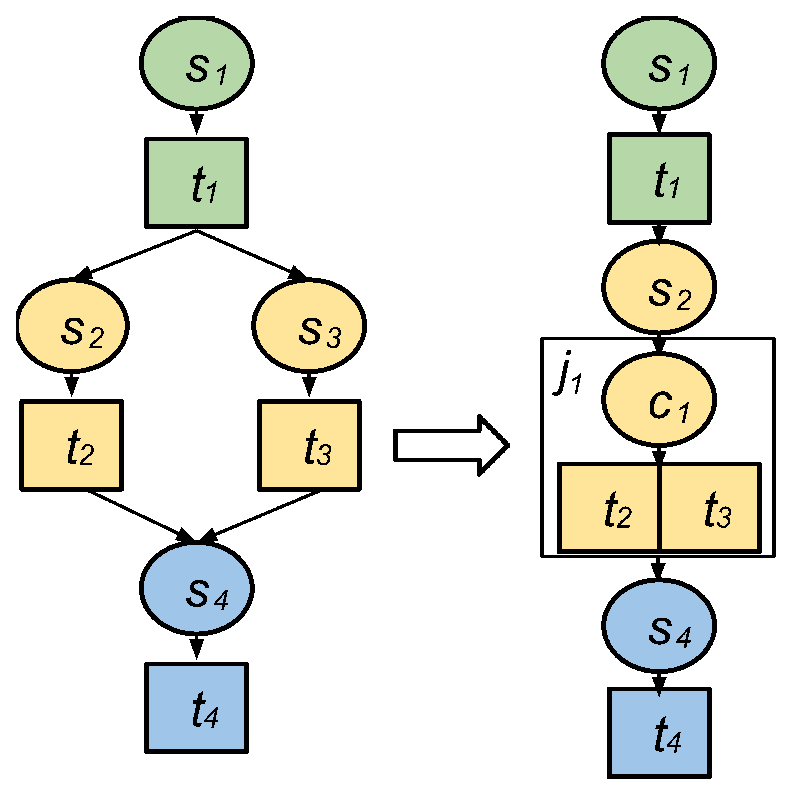
\includegraphics[width=0.5\linewidth]{figure3.eps}
  \captionof{figure}{An example of horizontal clustering (color indicates the horizontal level of a task).}
  \label{fig:model_hc}
\end{figure}

Figure~\ref{fig:model_vc} illustrates an example of vertical clustering, in which tasks $t_2$, $t_4$, and $t_6$ are merged into $j_1$, while tasks $t_3$, $t_5$, and $t_7$ are merged into $j_2$. Similarly, clustering delays $c_2$ and $c_3$ are added to $j_1$ and $j_2$ respectively, but system overheads $s_4$, $s_5$, $s_6$, and $s_7$ are removed. 




%Task clustering has been applied to many scenarios where resources are much less than tasks, which is true for many scientific workflows~\cite{Singh2008, Ying2009, Zomaya2004}, and has achieved significant improvement (i.e., 97\% as reported by ~\cite{Singh2008}) over the case without clustering. Table~\ref{tab:model_stats} shows the statistical workflow information (average task runtime etc. ) of six widely used scientific applications and their runtime information (number of nodes, average queue delay, etc.)~\cite{Chen2011}. For all of these workflows, there are a lot more tasks than available nodes and the average task runtime is shorted than system overheads. Therefore, task clustering can achieve significant improvement over no clustering. Besides the benefits of runtime improvement, task clustering also allows us to run on some federated distributed environment. For example, FutureGrid~\cite{FutureGrid} allows a user to use up to 20 VMs at a time. We will introduce the details of these workflows and distributed platforms in Session~\ref{sec:experiments}

%\begin{table*}[htbp]
%\centering
%\begin{tabular}{lrrrrrrrr}
%\hline
%Workflow & Venue & Nodes & Tasks & Workflow Engine Delay  &  Queue Delay  & Task Runtime  \\
%
%\hline
%
%SIPHT & UW Madison & 8 & 33 & 17 & 69 & 20\\ 
%Broadband & Amazon EC2 & 8 &770 & 17 &945&308\\
%Epigenomics &Amazon EC2&8& 83 &6&311&158\\
%CyberShake &Skynet&5&24142&12&188&5\\
%Montage &USC&20&10427&182&26136&523\\
%
%
%\hline
%\end{tabular}
%\caption{Overhead (in seconds) and Runtime Information }
%\label{tab:model_stats}
%\end{table*} 
 \section{Balanced Clustering}
\label{sec:imbalance}

Task clustering has been widely used to address the low performance of very short running tasks on platforms where the system overhead is high, such as distributed computing infrastructures. However, up to now, techniques do not consider the load balance problem. In particular, merging tasks within a workflow level without considering the runtime variance may cause load imbalance (Runtime Imbalance), or merging tasks without considering their data dependencies may lead to data locality problems (Dependency Imbalance). In this section, we introduce metrics that quantitatively capture workflow characteristics to measure runtime and dependence imbalances. We then present methods to handle the load balance problem.

\begin{figure}[!t]
\centering
 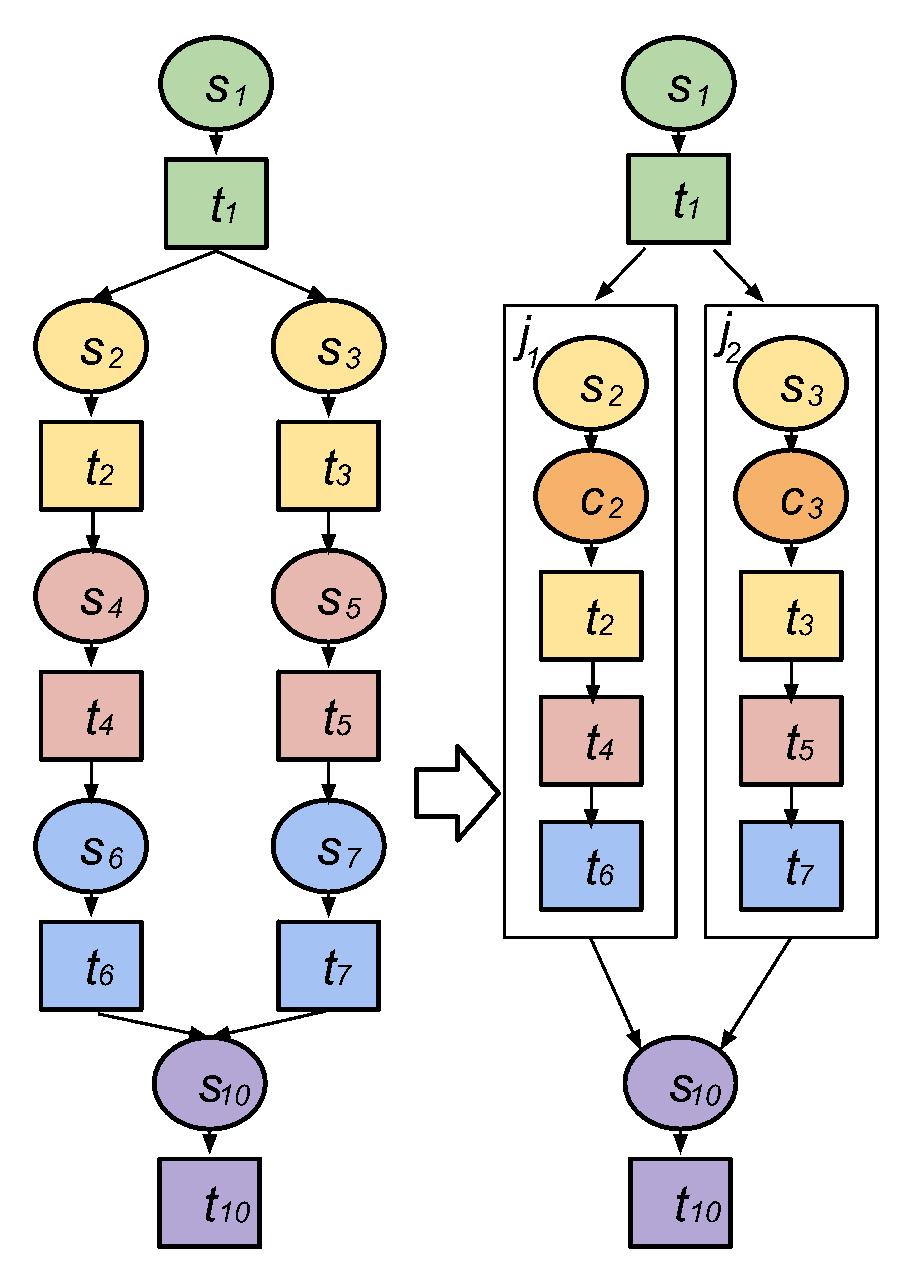
\includegraphics[width=0.55\linewidth]{figure4.eps}
  \captionof{figure}{An example of vertical clustering.}
  \label{fig:model_vc}
\end{figure}

\subsection{Imbalance metrics}

\textbf{Runtime Imbalance} describes the difference of the task/job runtime of a group of tasks/jobs. In this work, we denote the \textbf{Horizontal Runtime Variance} ($HRV$) as the ratio of the standard deviation in task runtime to the average runtime of tasks/jobs at the same horizontal level of a workflow. At the same horizontal level, the job with the longest runtime often controls the release of the next level jobs. A high $HRV$ value means that the release of next level jobs has been delayed. Therefore, to improve runtime performance, it makes sense to reduce the standard deviation of job runtime. Figure~\ref{fig:imbalance_rv} shows an example of four independent tasks $t_1$, $t_2$, $t_3$ and $t_4$ where the task runtime of $t_1$ and $t_2$ is 10 seconds, and the task runtime of $t_3$ and $t_4$ is 30 seconds. In the Horizontal Clustering (HC) approach, a possible clustering result could be {to merge }$t_1$ and $t_2$ into a clustered job, and $t_3$ and $t_4$ into another. This approach results in imbalanced runtime, i.e., $HRV > 0$ (Figure~\ref{fig:imbalance_rv}-top). In contrast, a balanced clustering strategy should try its best to evenly distribute task runtime among jobs as shown in Figure~\ref{fig:imbalance_rv} (bottom). A smaller \emph{HRV} means that the runtime of tasks within a horizontal level is more evenly distributed and therefore it is less necessary to use runtime-based balancing algorithms. However, runtime variance is not able to {capture }how symmetric the structure of the dependencies between tasks is.

\begin{figure}[htb]
	\centering
	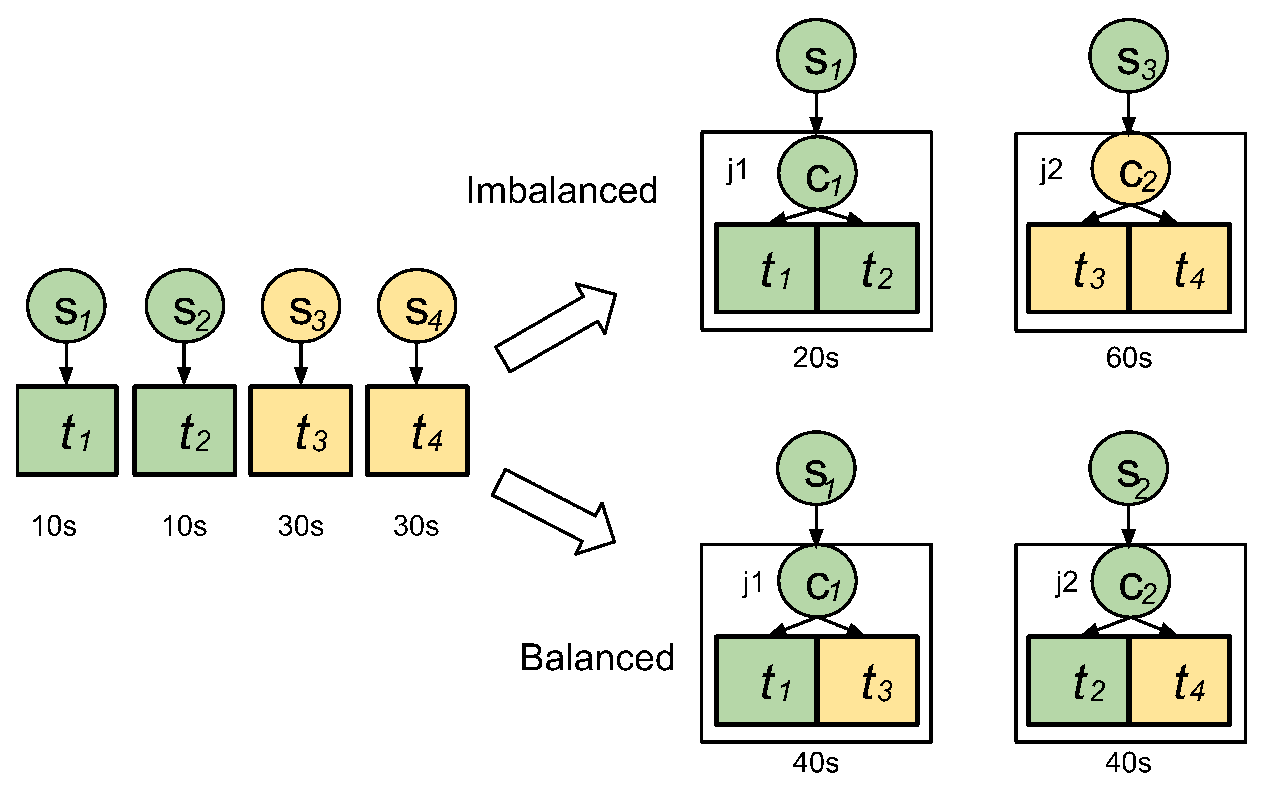
\includegraphics[width=0.95\linewidth]{figure5.eps}
	\captionof{figure}{An example of Horizontal Runtime Variance.}
	\label{fig:imbalance_rv}
\end{figure}


\textbf{Dependency Imbalance} means that the task clustering at one horizontal level forces the tasks at the next level (or even subsequent levels) to have severe data locality problems and thus loss of parallelism. For example, in Figure~\ref{fig:imbalance_dv}, we show a two-level workflow composed of four tasks in the first level and two in the second. Merging $t_1$ with $t_3$ and $t_2$ with $t_4$ (imbalanced workflow in Figure~\ref{fig:imbalance_dv}) forces $t_5$ and $t_6$ to transfer files from two locations and wait for the completion of $t_1$, $t_2$, $t_3$, and $t_4$.  A balanced clustering strategy groups tasks that have the maximum number of child tasks in common. Thus, $t_5$ can start to execute as soon as $t_1$ and $t_2$ are completed, and so can $t_6$. To {quantitatively measure }the Dependency Imbalance of a workflow, we propose two  metrics: ($i$) Impact Factor Variance, and ($ii$) Distance Variance. 

\begin{figure}[htb]
	\centering
	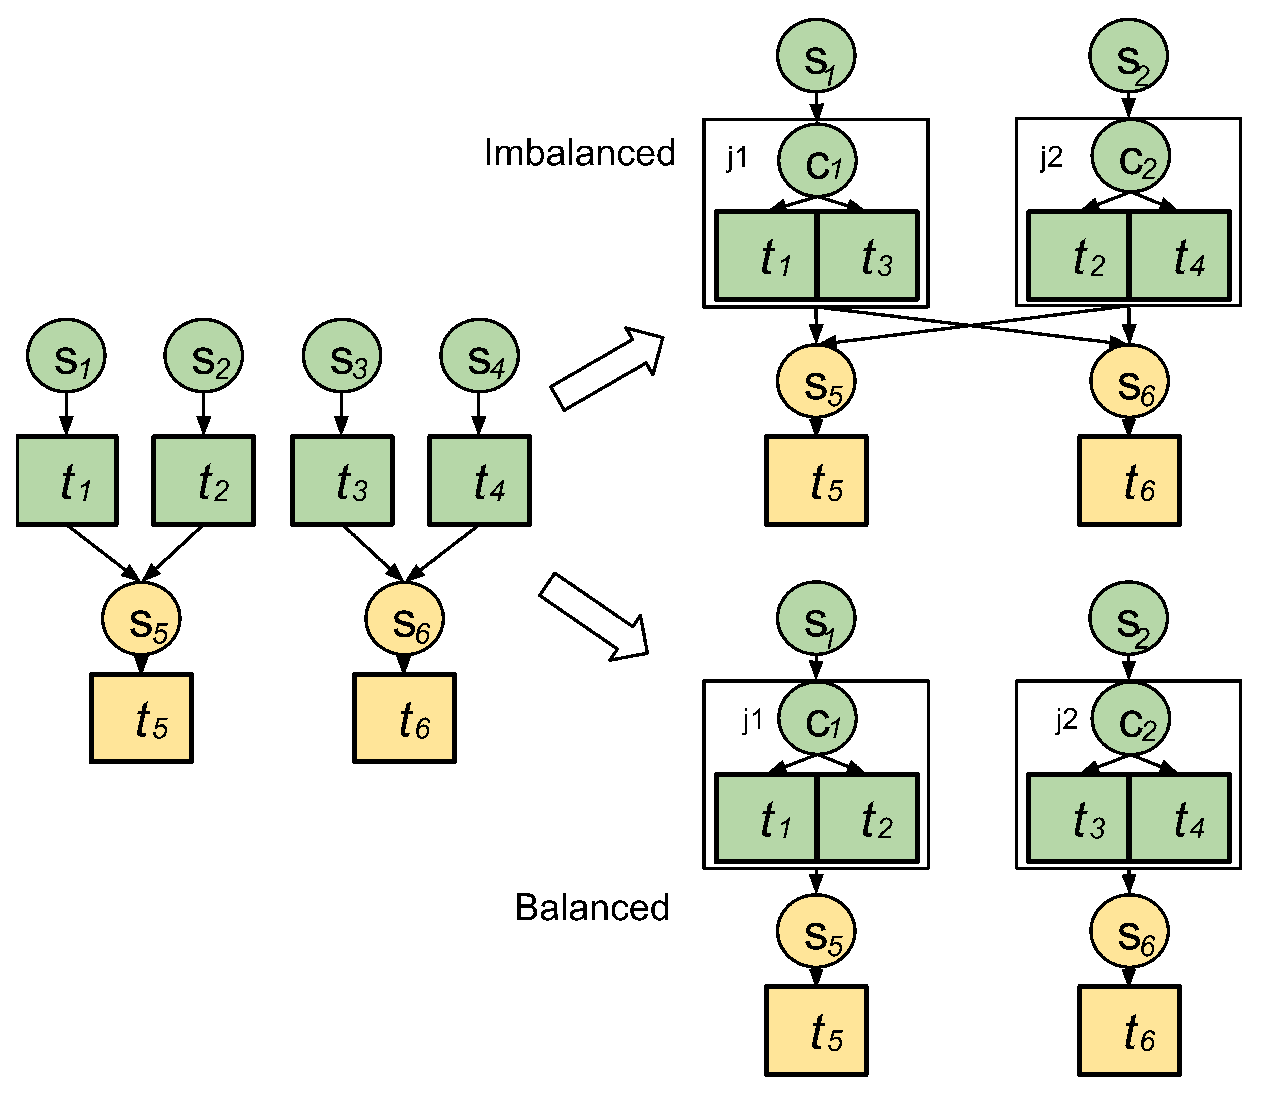
\includegraphics[width=0.95\linewidth]{figure6.eps}
	\captionof{figure}{An example of Dependency Imbalance.}
	\label{fig:imbalance_dv}
\end{figure}

We define the \textbf{Impact Factor Variance} ($IFV$) of tasks as the standard deviation of their impact factors. The \textbf{Impact Factor} ($IF$) of a task $t_u$ is defined as follows:

\begin{equation}
\label{eq:imbalance_impact_factor}
	IF(t_u)=\sum_{t_v\in Child(t_u)}^{}\frac{IF(t_v)}{||Parent(t_v)||}
\end{equation}
where $Child(t_u)$ denotes the set of child tasks of $t_u$, and $||Parent(t_v)||$ the number of parent tasks of $t_v$. The Impact Factor aims {to capture }the similarity of tasks/jobs in a graph by measuring their relative impact factor or importance to the entire graph. Tasks with similar impact factors are merged together, so that the workflow structure tends to be more {``even'' }or symmetric. For simplicity, we assume the $IF$ of a workflow exit task ({a task without children}, e.g. $t_5$ in Figure~\ref{fig:imbalance_dv}) is 1.0. {Consider }the two workflows presented in Figure~\ref{fig:imbalance_hifv}. The $IF$ for each of $t_1$, $t_2$, $t_3$, and $t_4$ is computed as follows:
\begin{eqnarray}
	\displaystyle  
	&IF(t_7 )=1.0, IF(t_6 )=IF(t_5 )=IF(t_7 )/2=0.5\nonumber  \\
	&IF(t_1 )=IF(t_2 )=IF(t_5 )/2=0.25\nonumber \\
	&IF(t_3 )=IF(t_4 )=IF(t_6 )/2=0.25\nonumber 
\end{eqnarray}
Thus, IFV($t_1$, $t_2$, $t_3$, $t_4$) = 0. In contrast, the $IF$ for $t_{1'}$, $t_{2'}$, $t_{3'}$, and $t_{4'}$ is:
\begin{eqnarray}
	\displaystyle  
	&IF(t_{7'})=1.0, IF(t_{6'})=IF(t_{5'})=IF(t_{1'})=IF(t_{7'})/2=0.5\nonumber \\
	&IF(t_{2'})=IF(t_{3'})=IF(t_{4'})=IF(t_{6'})/3=0.17 \nonumber
\end{eqnarray}
Therefore, the $IFV$ value for {$t_{1'}$, $t_{2'}$, $t_{3'}$, $t_{4'}$} is 0.17, which predicts {that }it is likely to be less symmetric than the workflow in Figure~\ref{fig:imbalance_hifv} (left). In this paper, we use \textbf{HIFV} (Horizontal IFV) to indicate the $IFV$ of tasks at the same horizontal level. The time complexity of calculating the $IF$ of all the tasks of a workflow with $n$ tasks is $O(n)$.  

\begin{figure}[htb]
	\centering
	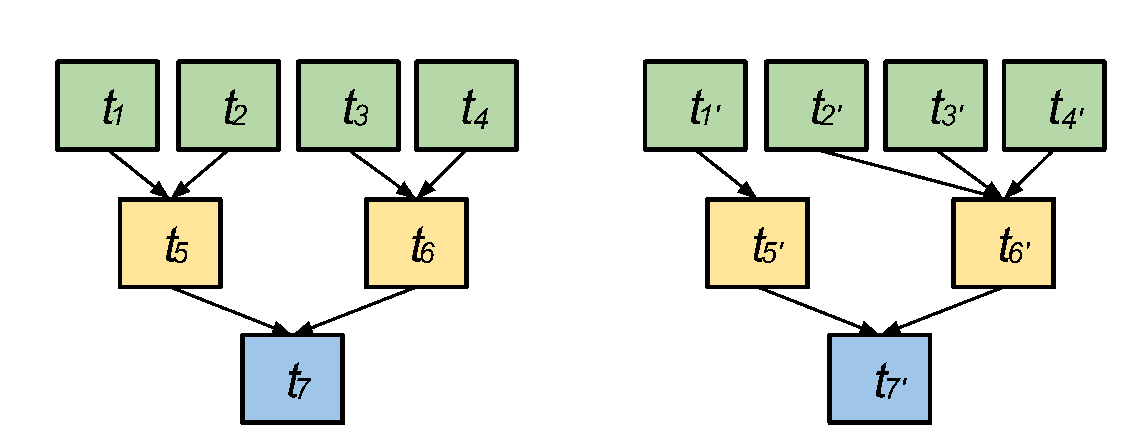
\includegraphics[width=0.85\linewidth]{figure7.eps}
	\captionof{figure}{Example of workflows with different data dependencies (For better visualization, we do not show system overheads in the rest of the paper).}
	\label{fig:imbalance_hifv}
\end{figure}

\textbf{Distance Variance} ($DV$) describes how `close' tasks are to each other. The distance between two tasks/jobs is defined as the {sum of the distance to }their closest common successor. If they do not have a common successor, the distance is set to infinity. For a group of $n$ tasks/jobs, the distance between them is represented by a $n \times n$ matrix $D$, where an element $D(u,v)$ denotes the distance between a pair of tasks/jobs $u$ and $v$. For any workflow structure, $D(u,v)=D(v,u)$ and $D(u,u)=0$, thus we ignore the cases when $u \geq v$. Distance Variance is then defined as the standard deviation of all the elements $D(u,v)$ for $u<v$. The time complexity of calculating all the values of $D$ of a workflow with $n$ tasks is $O(n^2)$. 

Similarly, $HDV$ indicates the $DV$ of a group of tasks/jobs at the same horizontal level. For example, Table~\ref{tab:imblance_metric} shows the distance matrices of tasks from the first level for both workflows of Figure~\ref{fig:imbalance_hifv} ($D_1$ for the workflow in the left, and $D_2$ for the workflow in the right). $HDV$ for $t_1, t_2, t_3$, and $t_4$ is 1.03, and for $t_{1'}, t_{2'}, t_{3'}$, and $t_{4'}$ is 1.10. In terms of distance variance, $D_1$ is more {``even'' }than $D_2$. A smaller $HDV$ means the tasks at the same horizontal level are more equally {``distant'' }from each other and thus the workflow structure tends to be more {``even'' }and symmetric. 

\begin{table}[htb]
	\footnotesize
	\centering
	\begin{tabular}{l|rrrr}
		$D_1$ & $t_1$ & $t_2$ & $t_3$ &$t_4$\\
		\hline
		$t_1$ & 0 & 2 & 4 & 4 \\
		$t_2$ & 2 & 0 & 4 & 4 \\
		$t_3$ & 4 & 4 & 0 & 2\\
		$t_4$ & 4 & 4 & 2 & 0 \\
	\end{tabular}
	\quad
	\begin{tabular}{l|rrrr}
		$D_2$ & $t_1'$ & $t_2'$ & $t_3'$ &$t_4'$\\
		\hline
		$t_1'$ & 0 & 4 & 4 & 4 \\
		$t_2'$ & 4 & 0 & 2 & 2 \\
		$t_3'$ & 4 & 2 & 0 & 2\\
		$t_4'$ & 4 & 2 & 2 & 0 \\
	\end{tabular}
	\caption{Distance matrices of tasks from the first level of workflows in Figure~\ref{fig:imbalance_hifv}.}
	\label{tab:imblance_metric}
\end{table}

In conclusion, runtime variance and dependency variance offer a quantitative and comparable tool to measure and evaluate the internal structure of a workflow. 



\subsection{Balanced clustering methods}
\label{sec:methods}
In this subsection, we introduce our balanced clustering methods used to improve the runtime and dependency balances in task clustering. We first {present }the basic runtime-based clustering method, and then two other balancing methods that address the dependency imbalance problem. %We use the metrics presented in the previous subsection to evaluate a given workflow to decide which balancing method(s) is(are) more appropriate. 

%Algorithm~\ref{alg:imbalance_algo} shows the pseudocode of our balanced clustering algorithm that uses a combination of these balancing methods and metrics.  The maximum number of clustered jobs (size of $CL$) is equal to the number of available resources multiplied by a \emph{clustering factor}. 

%\begin{algorithm}[htb]
%	\caption{ Balanced Clustering algorithm}
%	\footnotesize
%	\label{alg:imbalance_algo}
%	\begin{algorithmic}[1]
%		\Require $W$: workflow; $CL$: list of clustered jobs; $C$: the required size of $CL$; 
%		\Ensure The job runtime of $CL$ are as even as possible
%		\Procedure{Clustering}{$W,D,C$}
%			\State Sort $W$ in decreasing order of the size of each level
%			\For{$level < $the depth of $W$}
%				\State $TL\gets $\ \Call{GetTasksAtLevel}{$w,level$} \Comment{Partition $W$ based on depth}
%				\State $CL\gets$  \ \Call{Merge}{$TL,C$} \Comment{Form a list of clustered jobs}
%				\State $W \gets W - TL + CL$  \Comment{Merge dependencies as well} 
%			\EndFor
%		\EndProcedure
%		\Procedure{Merge}{$TL, C$}
%			\State Sort $TL$ in decreasing order of task runtime
%			\For{$t\ in\ TL$}
%				\State $J \gets $\ \Call{GetCandidateJob}{$CL, t$} \Comment{Get a candidate task}
%				\State  $J \gets J\ +\ t$ \Comment{Merge it with the clustered job}
%			\EndFor
%			\State \textbf{return} $CL$
%		\EndProcedure
%		\Procedure{GetCandidateJob}{$CL, t$}
%			\State Selects a job based on balanced clustering methods
%		\EndProcedure
%	\end{algorithmic}
%\end{algorithm}

%We examine tasks in a level-by-level approach starting from the level with the largest width (number of tasks at the same level, \texttt{line 2}). The intuition behind this breadth favored approach is that we believe it should improve the performance most. Then, we determine which type of imbalance problem a workflow experiences based on the balanced clustering metrics presented previously ($HRV$, $HIFV$, and $HDV$), and accordingly, we select a combination of balancing methods. \textsc{GetCandidateJob} selects a job (\texttt{line 12}) from a list of potential candidate jobs ($CL$) to be merged with the targeting task ($t$). Below we introduce the three balancing methods proposed in this work.


\begin{algorithm}[!htb]
	\footnotesize
	\caption{Horizontal Runtime Balancing algorithm.}
	\label{alg:imbalance_hrb}
	\begin{algorithmic}[1]
		\Require $W$: workflow; $R$: number of jobs per horizontal level
		\Procedure{Clustering}{$W,R$}
			\For{$level < depth(W)$}
				\State $TL\gets $\ \Call{GetTasksAtLevel}{$W,level$} \Comment{Partition $W$ based on depth}
				\State $C \gets TL.size() / R$ \Comment{$C$ is number of tasks per job in this level}
				\State $CL\gets$  \ \Call{Merge}{$TL,C, R$} \Comment{Returns a list of clustered jobs}
				\State $W \gets W - TL + CL$  \Comment{Merge dependencies as well} 
			\EndFor
		\EndProcedure
		\Procedure{Merge}{$TL, C, R$}
			\For{$i<R$}
			\State $J_i\gets$\{\}\Comment{An empty job}
			\EndFor
			\State $CL\gets$\{\}\Comment{An empty list of clustered jobs}
			\State Sort $TL$ in descending of runtime
			\ForAll{$t$ in $TL$}
				\State $J\gets$ the job with shortest runtime and less than $C$ tasks  
				\State $J$.add ($t$) \Comment{Adds the task to the shortest job}
				
			\EndFor
			\For{$i<R$}
			\State  $CL$.add( $J_i$)
			\EndFor
			\State \textbf{return} $CL$
		\EndProcedure
	\end{algorithmic}
\end{algorithm}



\textbf{Horizontal Runtime Balancing} (HRB) aims to evenly distribute task runtime among clustered jobs. Tasks with the longest runtime are added to the job with the shortest runtime. Algorithm~\ref{alg:imbalance_hrb} shows the pseudocode of HRB. This greedy method is used to address the load balance problem caused by runtime variance at the same horizontal level. Figure~\ref{fig:imbalance_hrb} shows an example of HRB where tasks in the first level have different runtimes and should be grouped into two jobs. HRB sorts tasks in decreasing order of runtime, and then adds the task with the highest runtime to the group with the shortest aggregated runtime. Thus, $t_1$ and $t_3$, as well as $t_2$ and $t_4$ are merged together.
For simplicity, system overheads are not displayed.

\begin{figure}[htb]
	\centering
	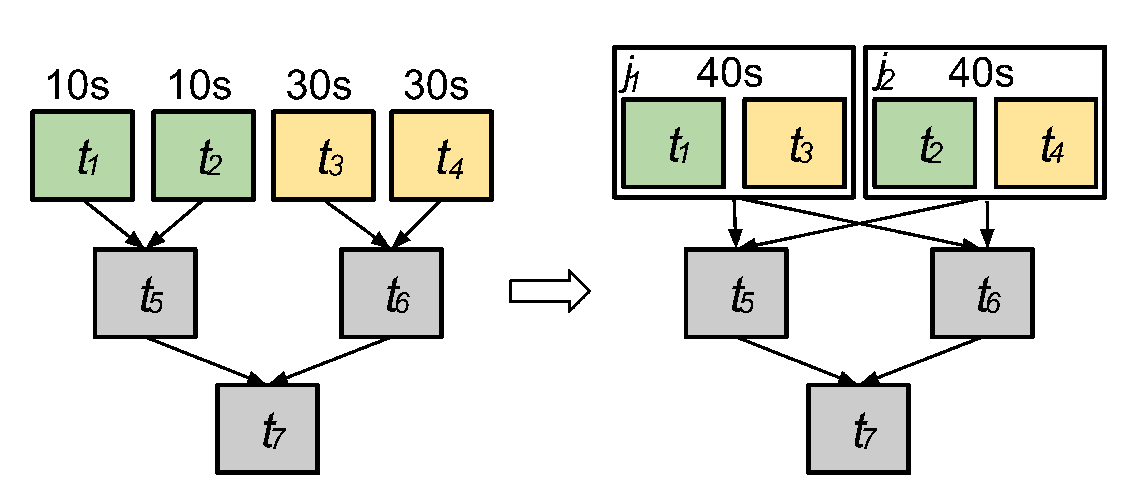
\includegraphics[width=0.85\linewidth]{figure8.eps}
	\caption{An example of the HRB (Horizontal Runtime Balancing) method. By solely addressing runtime variance, data locality problems may arise.}
	\label{fig:imbalance_hrb}
\end{figure}

\begin{algorithm}[!htb]
	\footnotesize
	\caption{Horizontal Impact Factor Balancing algorithm.}
	\label{alg:imbalance_hifb}
	\begin{algorithmic}[1]
		\Require $W$: workflow; $R$: number of jobs per horizontal level
		\Procedure{Clustering}{$W,R$}
			\For{$level < depth(W)$}
				\State $TL\gets $\ \Call{GetTasksAtLevel}{$W,level$} \Comment{Partition $W$ based on depth}
				\State $C \gets TL.size() / R$ \Comment{$C$ is number of tasks per job in this level}
				\State $CL\gets$  \ \Call{Merge}{$TL,C, R$} \Comment{Returns a list of clustered jobs}
				\State $W \gets W - TL + CL$  \Comment{Merge dependencies as well} 
			\EndFor
		\EndProcedure
		\Procedure{Merge}{$TL, C, R$}
			\For{$i<R$}
			\State $J_i\gets$\{\}\Comment{An empty job}
			\EndFor
			\State $CL\gets$\{\}\Comment{An empty list of clustered jobs}
			\State Sort $TL$ in descending of runtime
			\ForAll{$t$ in $TL$}
				\State $L\gets$ Sort all $J_i$ with the similarity of impact factors with $t$
				\State $J\gets$ the job with shortest runtime and less than $C$ tasks in $L$
				\State $J$.add ($t$) 
				
			\EndFor
			\For{$i<R$}
			\State  $CL$.add( $J_i$)
			\EndFor
			\State \textbf{return} $CL$
		\EndProcedure
	\end{algorithmic}
\end{algorithm}


\begin{algorithm}[!htb]
	\footnotesize
	\caption{Horizontal Distance Balancing algorithm.}
	\label{alg:imbalance_hdb}
	\begin{algorithmic}[1]
		\Require $W$: workflow; $R$: number of jobs per horizontal level
		\Procedure{Clustering}{$W,C$}
			\For{$level < depth(W)$}
				\State $TL\gets $\ \Call{GetTasksAtLevel}{$W,level$} \Comment{Partition $W$ based on depth}
				\State $C \gets TL.size() / R$ \Comment{$C$ is number of tasks per job in this level}
				\State $CL\gets$  \ \Call{Merge}{$TL,C, R$} \Comment{Returns a list of clustered jobs}
				\State $W \gets W - TL + CL$  \Comment{Merge dependencies as well} 
			\EndFor
		\EndProcedure
		\Procedure{Merge}{$TL, C, R$}
			\For{$i<R$}
			\State $J_i\gets$\{\}\Comment{An empty job}
			\EndFor
			\State $CL\gets$\{\}\Comment{An empty list of clustered jobs}
			\State Sort $TL$ in descending of runtime
			\ForAll{$t$ in $TL$}
				\State $L\gets$ Sort all $J_i$ with the closest distance with $t$
				\State $J\gets$ the job with shortest runtime and less than $C$ tasks in $L$
				\State $J$.add ($t$) 
				
			\EndFor
			\For{$i<R$}
			\State  $CL$.add( $J_i$)
			\EndFor
			\State \textbf{return} $CL$
		\EndProcedure
	\end{algorithmic}
\end{algorithm}


%how HRB works in an example of four jobs with different job runtime (assuming the height of a job is its runtime). For the given task ($t_0$), HRB sorts the potential jobs ($j_1$, $j_2$, $j_3$, and $j_4$) based on their runtime and selects the shortest job (in this case $j_1$ or $j_2$). 



However, HRB may cause a dependency imbalance problem since the clustering does not take data dependency into consideration. To address this problem, we propose the \textbf{Horizontal Impact Factor Balancing} (HIFB) and the \textbf{Horizontal Distance Balancing} (HDB) methods. 

In HRB, candidate jobs within a workflow level are sorted by their runtime, while in HIFB jobs are first sorted based on their similarity of $IF$, then {based }on runtime. 
Algorithm~\ref{alg:imbalance_hifb} shows the pseudocode of HIFB. 
For example, in Figure~\ref{fig:imbalance_hifb}, $t_1$ and $t_2$ have $IF = 0.25$, while $t_3$, $t_4$, and $t_5$ have $IF = 0.16$. HIFB selects a list of candidate jobs with the same IF value, and then HRB is performed to select the shortest job. Thus, HIFB merges $t_1$ and $t_2$ together, as well as $t_3$ and $t_4$.

\begin{figure}[htb]
	\centering
	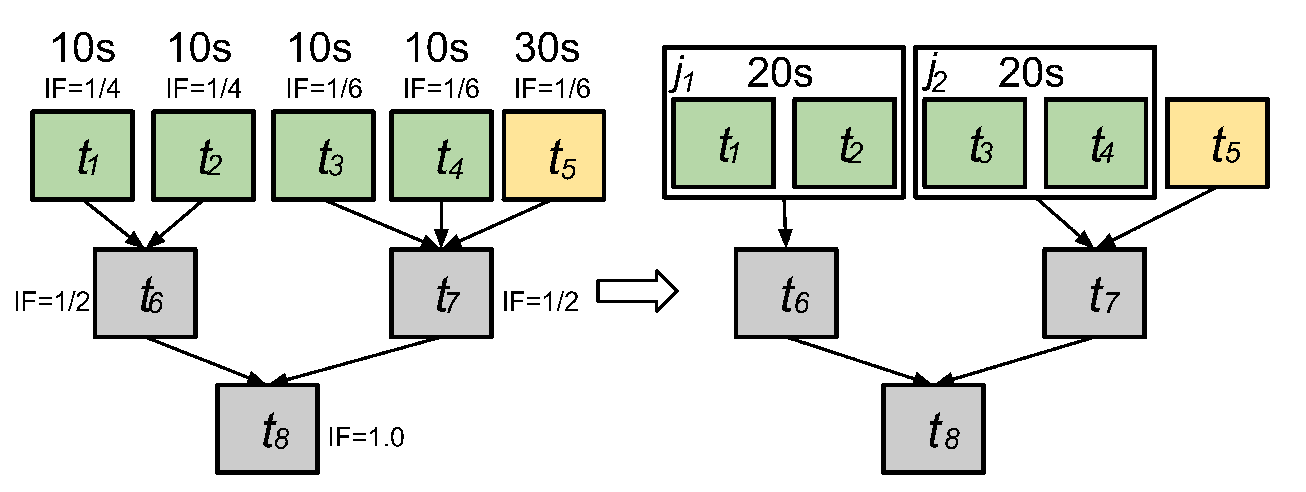
\includegraphics[width=\linewidth]{figure9.eps}
	\captionof{figure}{An example of the HIFB (Horizontal Impact Factor Balancing) method. Impact factors allow the detection of similarities between tasks.}
	\label{fig:imbalance_hifb}
\end{figure}

However, HIFB is {often }suitable for workflows with {an }asymmetric structure. A symmetric workflow structure means there exists a (usually vertical) division of the workflow graph such that one part of the workflow is a mirror of the other part. For symmetric workflows, such as the one shown in Figure~\ref{fig:imbalance_hrb}, the $IF$ value for all tasks of the first level will be the same ($IF=0.25$), thus the method may also cause dependency imbalance. In HDB, jobs are sorted based on the distance between them and the targeted task $t$, then on their runtimes. 
Algorithm~\ref{alg:imbalance_hdb} shows the pseudocode of HDB. 
For instance, in Figure~\ref{fig:imbalance_hdb}, the distances between tasks $D(t_1,t_2)=D(t_3,t_4)=2$, while $D(t_1,t_3)=D(t_1,t_4)=D(t_2,t_3)=D(t_2,t_4)=4$. Thus, HDB merges a list of candidate tasks with the minimal distance ($t_1$ and $t_2$, and $t_3$ and $t_4$). Note that even if the workflow is asymmetric (Figure~\ref{fig:imbalance_hifb}), HDB would obtain the same result as with HIFB. 

\begin{figure}[!htb]
	\centering
	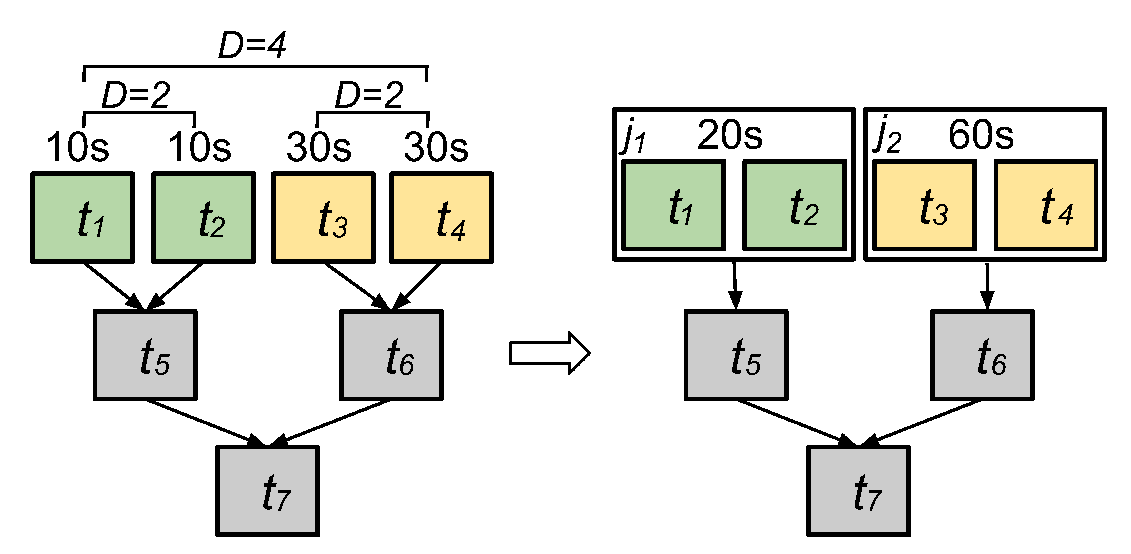
\includegraphics[width=0.85\linewidth]{figure10.eps}
	\captionof{figure}{An example of the HDB (Horizontal Distance Balancing) method. Measuring the distances between tasks avoids data locality problems.}
	\label{fig:imbalance_hdb}
\end{figure}

There are cases where HDB would yield lower performance than HIFB. For instance, let $t_1$, $t_2$, $t_3$, $t_4$, and $t_5$ be the set of tasks to be merged in the workflow presented in Figure~\ref{fig:imbalance_hifb_hdb}. HDB does not identify the difference in the number of parent/child tasks between the tasks, since $d(t_u,t_v) = 2, \forall u,v \in [1,5], u \neq v$. On the other hand, HIFB does distinguish {between } them since their impact factors are slightly different. Example of such scientific workflows include the LIGO Inspiral workflow~\cite{LIGO}, which is used in the evaluation of this paper (Section~\ref{sec:results}).

\begin{figure}[!htb]
	\centering
	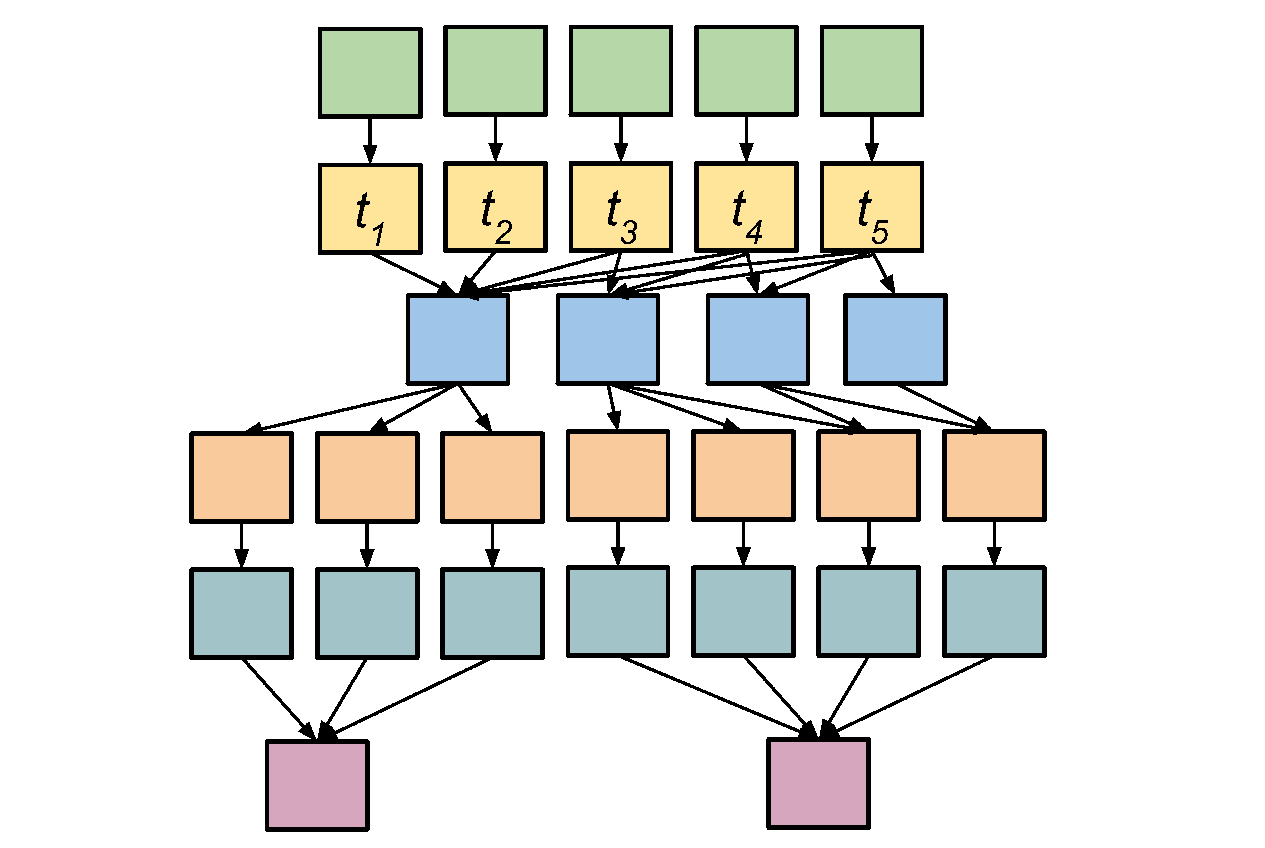
\includegraphics[width=0.85\linewidth]{figure11.eps}
	\captionof{figure}{A workflow example where HDB yields lower performance than HIFB. HDB does not capture the difference in the number of parents/child tasks, since the distances between tasks ($t_1$, $t_2$, $t_3$, $t_4$, and $t_5$) are the same.}
	\label{fig:imbalance_hifb_hdb}
\end{figure}

%In conclusion,  
Table~\ref{tab:2} summarizes the imbalance metrics and balancing methods introduced in this section. These balancing methods have different preference{s when selecting }a candidate job to be merged. For instance, HIFB tends to group tasks that share similar importance to the workflow structure, while HDB tends to group tasks that reduce data transfers.

\begin{figure}[htb]
	\centering
	\small
	\begin{tabular}{l|l}
		\hline
		\textbf{Imbalance Metrics} & $abbr.$   \\
		\hline
		Horizontal Runtime Variance & \emph{HRV}   \\ 
%		%Pipeline Runtime Variance &{\em PRV}  \\ 
		Horizontal Impact Factor Variance & \emph{HIFV} \\ 
		Horizontal Distance Variance & \emph{HDV}  \\ 
		\hline
		\textbf{Balancing Methods} & $abbr.$  \\
		\hline
%		Horizontal Clustering & HC \\
		Horizontal Runtime Balancing & HRB   \\ 
%		Vertical Clustering & VC \\ 
		Horizontal Impact Factor Balancing & HIFB\\ 
		Horizontal Distance Balancing & HDB \\ 
		\hline
	\end{tabular}
	\captionof{table}{Summary of imbalance metrics and balancing methods.}
	\label{tab:2}
\end{figure}



\subsection{Combining vertical clustering methods}

In this subsection, we discuss how we combine the balanced clustering methods presented above with vertical clustering (VC).
%For one example workflow shown in Figure~\ref{fig:imbalance_vc}, we may simply merge tasks at the fourth level and tasks at the fifth level vertically. 
In pipelined workflows (single-parent-single-child tasks), vertical clustering always yields improvement over a baseline, non-clustered execution because merging reduces system overheads and data transfers within the pipeline. Horizontal clustering does not have the same guarantee since its performance depends on the comparison of system overheads and task durations. However, vertical clustering has {a }limited performance improvement if the workflow does not have pipelines. Therefore, we are interested in the analysis of the performance impact of applying both vertical and horizontal clustering in the same workflow. We combine these methods in two ways: (\emph{i}) \emph{VC-prior}, and (\emph{ii}) \emph{VC-posterior}.


%\label{sec:vertical}
%\begin{figure}[htb]
%	\centering
%	\includegraphics[width=0.35\linewidth]{figures/imbalance/vertical_clustering.eps}
%	\captionof{figure}{An example of Vertical Clustering.}
%	\label{fig:imbalance_vc}
%\end{figure}

\paragraph{\textbf{VC-prior}}
In this method, vertical clustering is performed first, and then the balancing methods (HRB, HIFB, HDB, or HC) are applied. Figure~\ref{fig:imbalance_vc_prior} shows an example where pipelined-tasks are merged first, and then the merged pipelines are horizontally clustered based on the runtime variance.

\begin{figure}[!htb]
	\centering
	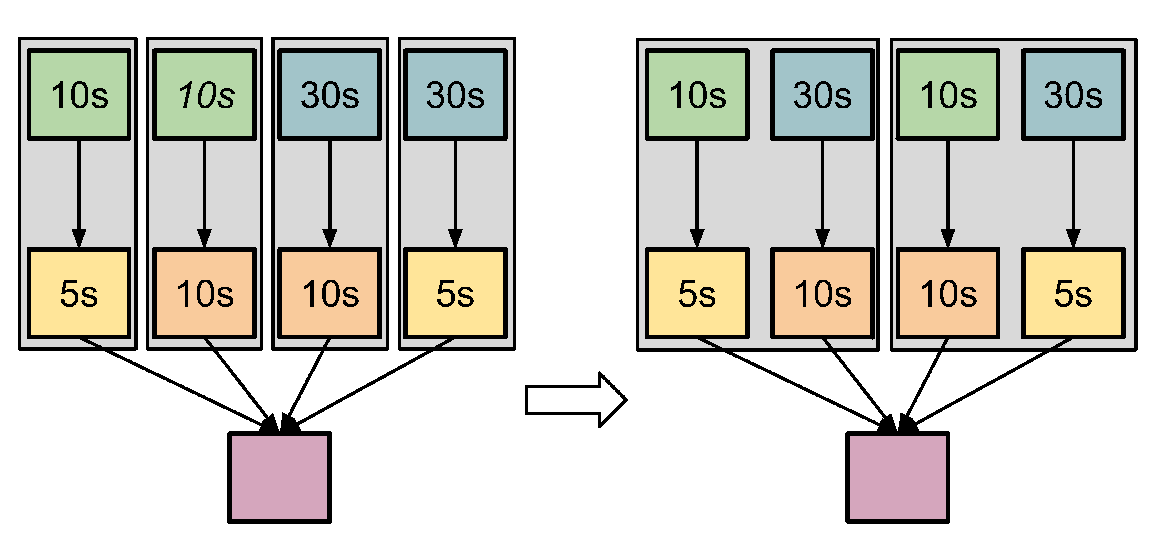
\includegraphics[width=0.85\linewidth]{figure12.eps}
	\captionof{figure}{\emph{VC-prior}: vertical clustering is performed first, and then the balancing methods.}
	\label{fig:imbalance_vc_prior}
\end{figure}

\paragraph{\textbf{VC-posterior}} 
%Here, vertical clustering is performed \emph{a posteriori}, i.e. balancing methods are first applied, and then VC. Figure~\ref{fig:imbalance_vc_posterior} shows an example where tasks are horizontally clustered first based on the runtime variance, and then merged vertically. In this example, vertical clustering targeted the data locality problem by merging tasks that would not generate interdependency once clustered. However, this approach causes a runtime imbalance problem.

\begin{figure}[!htb]
	\centering
	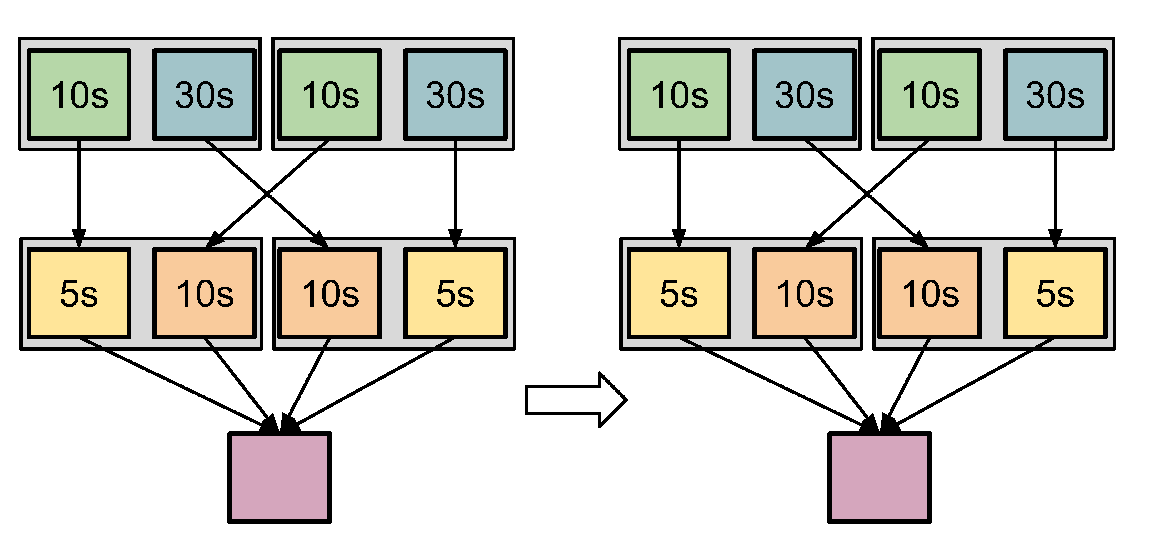
\includegraphics[width=0.85\linewidth]{figure13.eps}
	\captionof{figure}{\emph{VC-posterior}: horizontal clustering (balancing methods) is performed first, and then vertical clustering (but without changes).}
	\label{fig:imbalance_vc_posterior}
\end{figure}

Here, {horizontal }balancing methods are first applied, and then vertical clustering {is performed}. Figure~\ref{fig:imbalance_vc_posterior} shows an example where tasks are horizontally clustered first based on the runtime variance, and then merged vertically. However, since the original pipeline structures have been broken by horizontal clustering, VC does not perform any changes to the workflow. 


%means we perform horizontal clustering methods first and then vertical clustering. For the same workflow, assuming we merge tasks horizontally as shown in , we can see that we cannot perform vertical clustering to clustered jobs at the fourth level and the fifth level since the original pipeline structures have been destroyed by horizontal clustering. This phenomenon suggests us VC-posterior may work better compared to VC-prior, generally speaking. However, some opposite cases do exist. We will verify our hypothesis in Section~\ref{sec:results}. We will also compared the two combining approaches with \textbf{VC-only}, which means we perform vertical clustering only and \textbf{No-VC}, which means we just perform horizontal clustering methods without vertical clustering. 






% Section
\section{Evaluation}
\label{sec:experiments}

The experiments presented hereafter evaluate the performance of our balancing methods when compared to an existing and effective task clustering strategy named Horizontal Clustering (HC)~\cite{Singh:2008:WTC:1341811.1341822}, which is widely used by workflow management systems such as Pegasus~\cite{Deelman2004}. We also compare our methods with two heuristics described in literature: DFJS~\cite{Muthuvelu:2005:DJG:1082290.1082297}, and AFJS~\cite{Liu2009}. DFJS groups bags of tasks based on the task durations up to the resource capacity. AFJS is an extended version of DFJS that is an adaptive fine-grained job scheduling algorithm to group fine-grained tasks according to processing capacity of the current available resources and bandwidth between these resources.

% Workflow applications
\subsection{Scientific workflow applications}
\label{sec:applications}

Five real scientific workflow applications are used in the experiments: LIGO Inspiral analysis~\cite{LIGO}, Montage~\cite{Berriman2004}, CyberShake~\cite{Graves2010}, Epigenomics~\cite{Epigenome}, and SIPHT~\cite{SIPHT}. In this subsection, we describe each workflow application and present their main characteristics and structures.

\paragraph{\textbf{LIGO}}
Laser Interferometer Gravitational Wave Observatory (LIGO)~\cite{LIGO} workflows are used to search for gravitational wave signatures in data collected by large-scale interferometers. The observatories' mission is to detect and measure gravitational waves predicted by general relativity (Einstein's theory of gravity), in which gravity is described as due to the curvature of the fabric of time and space. The LIGO Inspiral workflow is a data-intensive workflow. Figure~\ref{fig:evaluation_shape_ligo} shows a simplified version of this workflow. The LIGO Inspiral workflow is separated into multiple groups of interconnected tasks, which we call branches in the rest of our paper. However, each branch may have a different number of pipelines as shown in Figure~\ref{fig:evaluation_shape_ligo}. 

\begin{figure}[!htb]
	\centering
	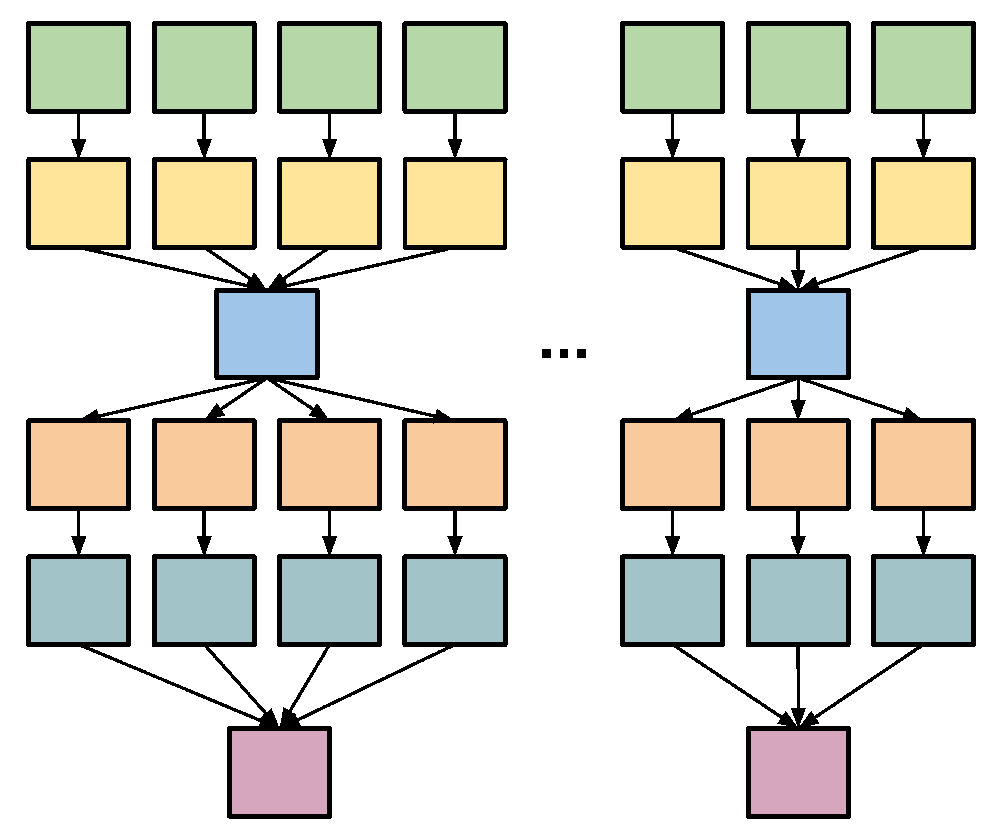
\includegraphics[width=0.5\linewidth]{figure14.eps} \\
	\caption{A simplified visualization of the LIGO Inspiral workflow.}
	\label{fig:evaluation_shape_ligo}
\end{figure}

\paragraph{\textbf{Montage}}
Montage~\cite{Berriman2004} is an astronomy application that is used to construct large image mosaics of the sky. Input images are reprojected onto a sphere and overlap is calculated for each input image. The application re-projects input images to the correct orientation while keeping background emission level constant in all images. The images are added by rectifying them to a common flux scale and background level. Finally{, }the reprojected images are co-added into a final mosaic. The resulting mosaic image can provide a much deeper and detailed understanding of the portion of the sky in question. Figure~\ref{fig:evaluation_shape_montage} illustrates a small Montage workflow. The size of the workflow depends on the number of images used in constructing the desired mosaic of the sky. The structure of the workflow changes to accommodate increases in the number of inputs, which corresponds to an increase in the number of computational tasks.

\begin{figure}[htb]
	\centering
	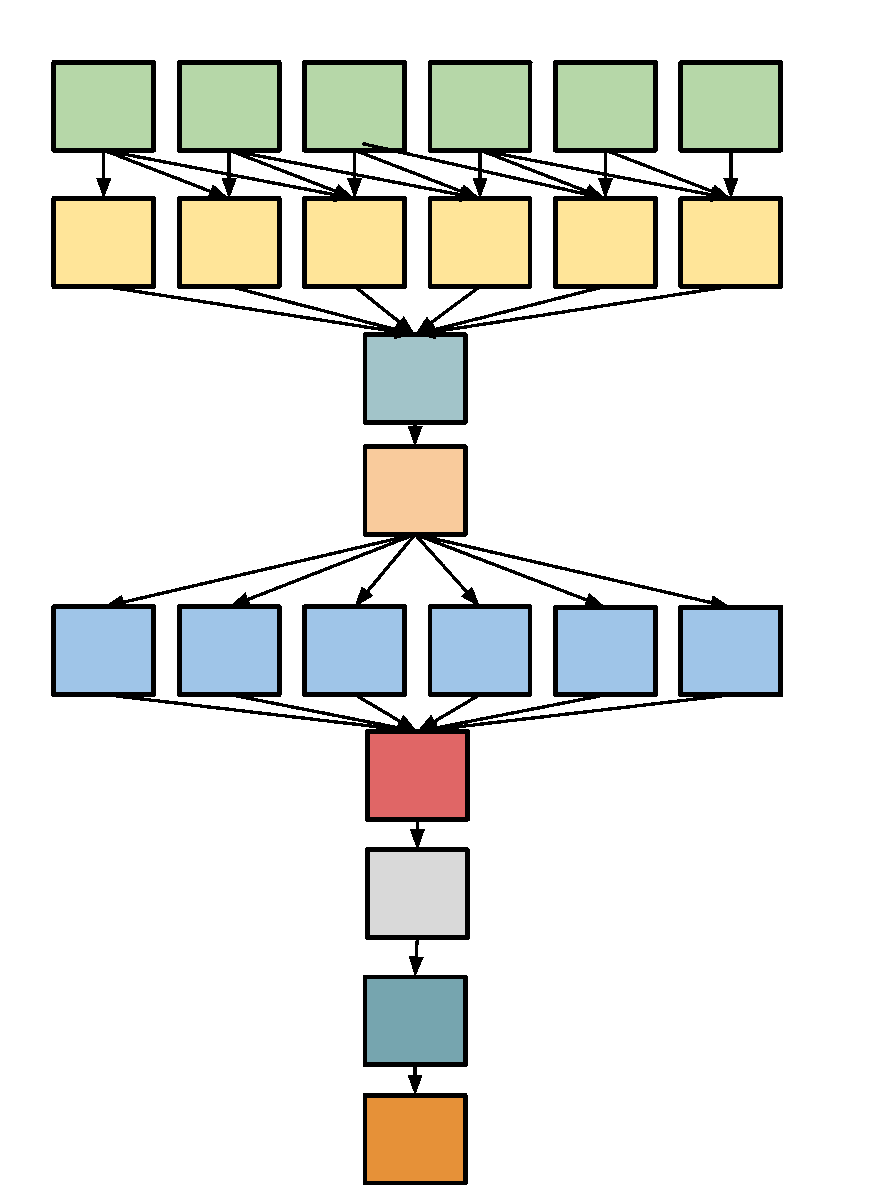
\includegraphics[width=0.4\linewidth]{figure15.eps} \\
	\caption{A simplified visualization of the Montage workflow.}
	\label{fig:evaluation_shape_montage}
\end{figure}

\paragraph{\textbf{Cybershake}}
CyberShake~\cite{Graves2010} is a seismology application that calculates Probabilistic Seismic Hazard curves for geographic sites in the Southern California region. It identifies all ruptures within 200km of the site of interest and converts rupture definition into multiple rupture variations with differing hypocenter locations and slip distributions. It then calculates synthetic seismograms for each rupture variance, and peak intensity measures are then extracted from these synthetics and combined with the original rupture probabilities to produce probabilistic seismic hazard curves for the site. Figure~\ref{fig:evaluation_shape_cybershake} shows an illustration of the Cybershake workflow.

\begin{figure}[htb]
	\centering
	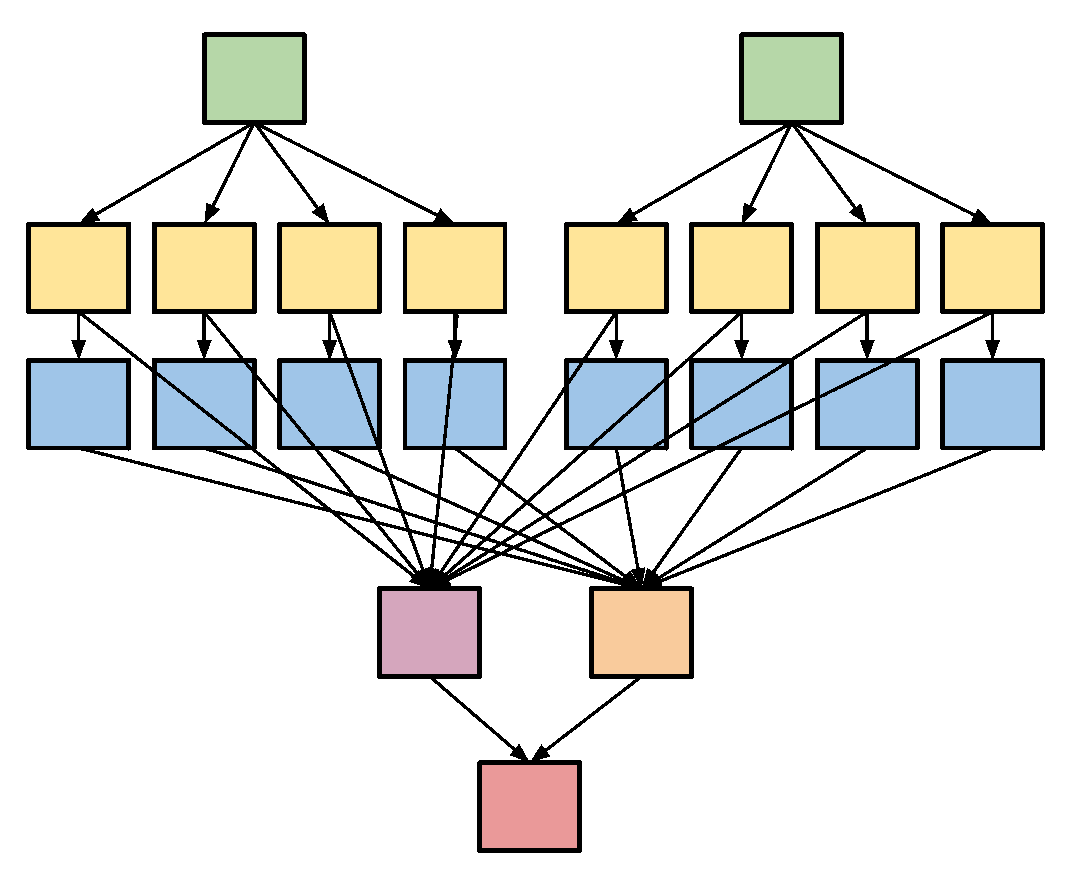
\includegraphics[width=0.55\linewidth]{figure16.eps} \\
	\caption{A simplified visualization of the CyberShake workflow.}
	\label{fig:evaluation_shape_cybershake}
\end{figure}

\paragraph{\textbf{Epigenomics}}
The Epigenomics workflow~\cite{Epigenome} is a data-parallel workflow. Initial data are acquired from the Illumina-Solexa Genetic Analyzer in the form of DNA sequence lanes. Each Solexa machine can generate multiple lanes of DNA sequences. These data are converted into a format that can be used by sequence mapping software. The mapping software can do one of two major tasks. It either maps short DNA reads from the sequence data onto a reference genome, or it takes all the short reads, treats them as small pieces in a puzzle and then tries to assemble an entire genome. In our experiments, the workflow maps DNA sequences to the correct locations in a reference Genome. This generates a map that displays the sequence density showing how many times a certain sequence expresses itself on a particular location on the reference genome. Epigenomics is a CPU-intensive application and its simplified structure is shown in Figure~\ref{fig:evaluation_shape_genome}. Different to the LIGO Inspiral workflow, each branch in Epigenomics has exactly the same number of pipelines, which makes it more symmetric. 

\begin{figure}[htb]
	\centering
	\includegraphics[width=.85\linewidth]{figure17.eps} \\
	\caption{A simplified visualization of the Epigenomics workflow with multiple branches.}
	\label{fig:evaluation_shape_genome}
\end{figure}

\paragraph{\textbf{SIPHT}}
The SIPHT workflow~\cite{SIPHT} conducts a wide search for small untranslated RNAs (sRNAs) that regulates several processes such as secretion or virulence in bacteria. The kingdom-wide prediction and annotation of sRNA encoding genes involves a variety of individual programs that are executed in the proper order using Pegasus~\cite{Deelman2004}. These involve the prediction of $\rho$-independent transcriptional terminators, BLAST (Basic Local Alignment Search Tools) comparisons of the inter genetic regions of different replicons and the annotations of any sRNAs that are found. A simplified structure of the SIPHT workflow is shown in Figure~\ref{fig:evaluation_shape_sipht}. 

\begin{figure}[htb]
	\centering
	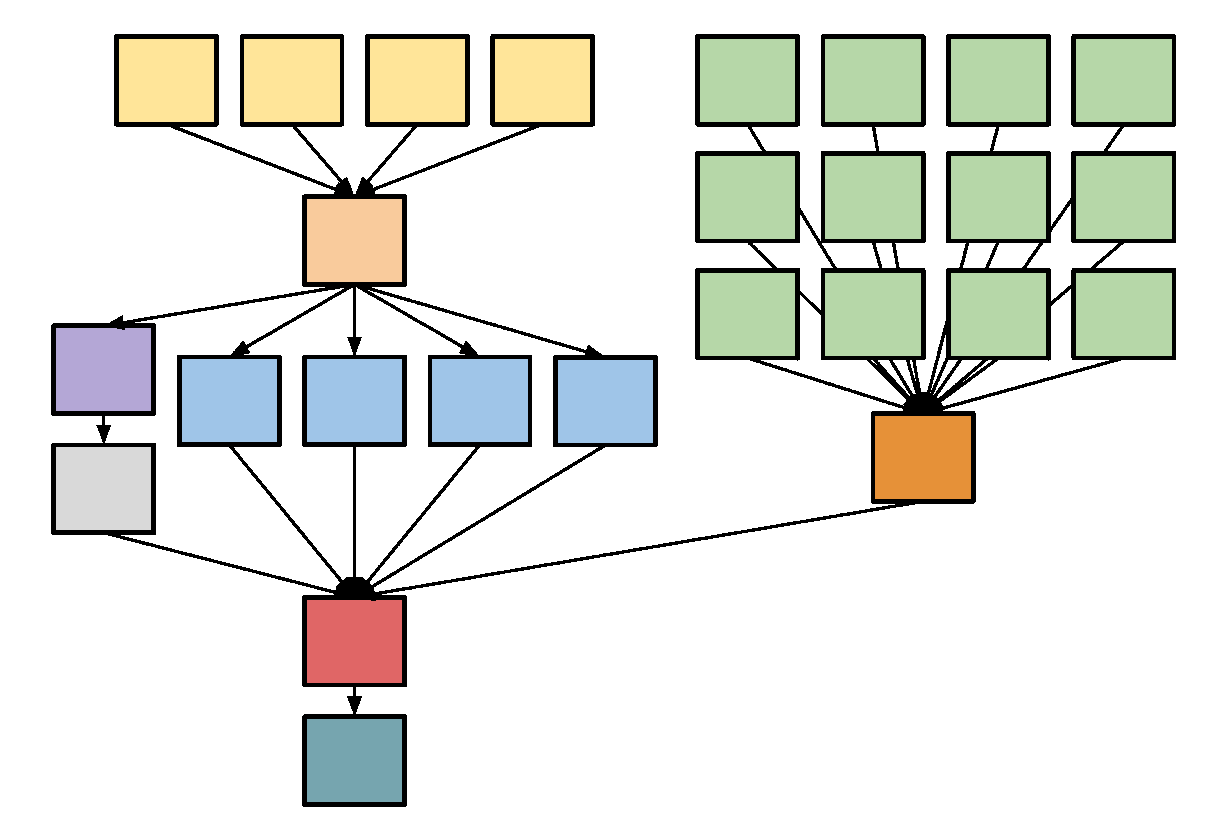
\includegraphics[width=0.6\linewidth]{figure18.eps} \\
	\caption{A simplified visualization of the SIPHT workflow.}
	\label{fig:evaluation_shape_sipht}
\end{figure}


\begin{table}[!htb]
	\setlength{\tabcolsep}{11pt}
	\centering
	\small
	\begin{tabular}{lrrrr}
		\hline
		 & \multicolumn{1}{c}{Number} & \multicolumn{1}{c}{Average} &  \multicolumn{1}{c}{Average} \\
		Workflow	& of Tasks	 & Data Size & Task Runtime \\
		\hline
		LIGO 		&800		& 5 MB	& 228s\\
		Montage 		&300		&3 MB	&11s\\
		CyberShake 	&700		&148 MB 	& 23s\\
		Epigenomics 	&165 	& 355 MB	& 2952s\\
		SIPHT		&1000	& 360 KB 	& 180s\\
		\hline
	\end{tabular}
	\caption{Summary of the scientific workflows characteristics.}
	\label{tab:evaluation_workflows}
\end{table} 

Table~\ref{tab:evaluation_workflows} shows the summary of the main \textbf{workflows characteristics}: number of tasks, average data size, and average task runtimes for the five workflows. {More detailed characteristics could be found in~\cite{Juve2013}}. 


% Task clustering techniques
\subsection{Task clustering techniques}

{The experiments }compare the performance of our balancing methods to the Horizontal Clustering (HC)~\cite{Singh:2008:WTC:1341811.1341822} technique, and with two methods well known from the literature, DFJS~\cite{Muthuvelu:2005:DJG:1082290.1082297} and AFJS~\cite{Liu2009}. In this subsection, we briefly describe each of these algorithms.


\paragraph{\textbf{HC}}
Horizontal Clustering (HC) merges multiple tasks that are at the same horizontal level of the workflow. The clustering granularity (number of tasks within a cluster) of a clustered job is controlled by the user, who defines either the number of tasks per clustered job (\emph{clusters.size}), or the number of clustered jobs per horizontal level of the workflow (\emph{clusters.num}). This algorithm has been implemented and used in Pegasus~\cite{Singh:2008:WTC:1341811.1341822}. For simplicity, we define \emph{clusters.num} as the number of available resources. In our prior work~\cite{6683907}, we have compared the runtime performance with different clustering granularity. The pseudocode of the HC technique is shown in Algorithm~\ref{alg:evaluation_hc}. 


\begin{algorithm}[!htb]
	\footnotesize
	\caption{Horizontal Clustering algorithm.}
	\label{alg:evaluation_hc}
	\begin{algorithmic}[1]
		\Require $W$: workflow; $C$: max number of tasks per job defined by \emph{clusters.size} or \emph{clusters.num}
		\Procedure{Clustering}{$W,C$}
			\For{$level < depth(W)$}
				\State $TL\gets $\ \Call{GetTasksAtLevel}{$W,level$} \Comment{Partition $W$ based on depth}
				\State $CL\gets$  \ \Call{Merge}{$TL,C$} \Comment{Returns a list of clustered jobs}
				\State $W \gets W - TL + CL$  \Comment{Merge dependencies as well} 
			\EndFor
		\EndProcedure
		\Procedure{Merge}{$TL, C$}
			\State $J\gets$ \{\}\Comment{An empty job}
			\State $CL\gets$\{\}\Comment{An empty list of clustered jobs}
			\While{$TL$ is not empty}
				\State $J$.add ($TL$.pop($C$) \Comment{Pops $C$ tasks that are not merged }
				\State  $CL$.add( $J$)
			\EndWhile
			\State \textbf{return} $CL$
		\EndProcedure
	\end{algorithmic}
\end{algorithm}

\paragraph{\textbf{DFJS}}
The dynamic fine-grained job scheduler (DFJS) was proposed by Muthuvelu et al.~\cite{Muthuvelu:2005:DJG:1082290.1082297}. The algorithm groups bags of tasks based on their granularity size---defined as the processing time of the task on the resource. Resources are ordered by their decreasing values of capacity (in MIPS), and tasks are grouped up to the resource capacity. This process continues until all tasks are grouped and assigned to resources. Algorithm~\ref{alg:evaluation_dfjs} shows the pseudocode of the heuristic. 
 
\begin{algorithm}[!htb]
	\caption{ DFJS algorithm.}
	\footnotesize
	\label{alg:evaluation_dfjs}
	\begin{algorithmic}[1]
		\Require $W$: workflow; $max.runtime$: max runtime of clustered jobs 
		\Procedure{Clustering}{$W,max.runtime$}
			\For{$level < $the depth of $W$}
				\State $TL\gets $\ \Call{GetTasksAtLevel}{$W,level$} \Comment{Partition $W$ based on depth}
				\State $CL\gets$  \ \Call{Merge}{$TL,max.runtime$} \Comment{Returns a list of clustered jobs}
				\State $W \gets W - TL + CL$  \Comment{Merge dependencies as well} 
			\EndFor
		\EndProcedure
		\Procedure{Merge}{$TL, max.runtime$}
			\State $J\gets$ \{\}\Comment{An empty job}
			\State $CL\gets$\{\}\Comment{An empty list of clustered jobs}
			\While{$TL$ is not empty}
				\State $t \gets TC$.pop() \Comment{Get a task that is not mereged}
				\If {$J$.runtime + $t$.runtime $> max.runtime$}
				\State	$CL$.add($J$)
				\State	$J \gets$\{\}
				\EndIf	
				\State $J$.add($t$)
			\EndWhile
			\State \textbf{return} $CL$
		\EndProcedure
	\end{algorithmic}
\end{algorithm}


\paragraph{\textbf{AFJS}}
The adaptive fine-grained job scheduler (AFJS)~\cite{Liu2009} is an extension of DFJS. It groups tasks not only based on the maximum runtime defined per cluster job, but also on the maximum data size per clustered job. The algorithm adds tasks to a clustered job until the job's runtime is greater than the maximum runtime or the job's total data size (input + output) is greater than the maximum data size. The AFJS heuristic pseudocode is shown in Algorithm~\ref{alg:evaluation_afjs}. 

\begin{algorithm}[!htb]
	\caption{ AFJS algorithm.}
	\footnotesize
	\label{alg:evaluation_afjs}
	\begin{algorithmic}[1]
		\Require $W$: workflow; $max.runtime$: the maximum runtime for a clustered jobs; $max.datasize$: the maximum data size for a clustered job
		\Procedure{Clustering}{$W,max.runtime$}
			\For{$level < $the depth of $W$}
				\State $TL\gets $\ \Call{GetTasksAtLevel}{$W,level$} \Comment{Partition $W$ based on depth}
				\State $CL\gets$  \ \Call{Merge}{$TL,max.runtime, max.datasize$} \Comment{Returns a list of clustered jobs}
				\State $W \gets W - TL + CL$  \Comment{Merge dependencies as well} 
			\EndFor
		\EndProcedure
		\Procedure{Merge}{$TL, max.runtime, max.datasize$}
			\State $J\gets$ \{\}\Comment{An empty job}
			\State $CL\gets$\{\}\Comment{An empty list of clustered jobs}
			\While{$TL$ is not empty}
				\State $t \gets TC$.pop() \Comment{Get a task that is not mereged}
				\If {$J$.runtime + $t$.runtime $> max.runtime$ OR $J$.datasize + $t$.datasize $> max.datasize$}
				\State	$CL$.add($J$)
				\State	$J \gets$\{\}
				\EndIf	
				\State $J$.add($t$)
			\EndWhile
			\State \textbf{return} $CL$
		\EndProcedure
	\end{algorithmic}
\end{algorithm}

DFJS and AFJS require parameter tuning (e.g. maximum runtime per clustered job) to efficiently cluster tasks into coarse-grained jobs. For instance, if the maximum runtime is too high, all tasks may be grouped into a single job, leading to loss of parallelism. In contrast, if the runtime threshold is too low, the algorithms do not group tasks, leading to no improvement over a baseline execution. 

For comparison purposes, we perform{ed }a parameter study in order to tune the algorithms for each workflow application described in Section~\ref{sec:applications}. Exploring all possible parameter combinations is a cumbersome and exhaustive task. In the original DFJS and AFJS works, these parameters are empirically chosen, however this approach requires deep knowledge {of }the workflow applications. Instead, we performed a parameter tuning study, where we first estimate{d }the upper bound of \emph{max.runtime} ($n$) as the sum of all task runtimes, and the lower bound of \emph{max.runtime} ($m$) as 1 second for simplicity. Data points {were }divided into ten chunks and then we sample one data point from each chunk. We then select{ed }the chunk that has the lowest makespan and set $n$ and $m$ as the upper and lower bounds of the selected chunk, respectively. These steps {were }repeated until $n$ and $m$ {had }converged into a data point.

%We do not provide a mathematical proof of the correctness of our method, since we are not focused on demonstrating the optimal tuning for DFJS and AFJS algorithms, but a rough estimation of the minimal makespan. Instead, 

To demonstrate the correctness of our sampling approach in practice, we show the relationship between the makespan and the \emph{max.runtime} for an example Montage workflow application in Figure~\ref{fig:evaluation_dfjs_montage}---experiment conditions are presented in Section~\ref{sec:experiment_conditions}. Data points are divided into 10 chunks of 250s each (for \emph{max.runtime}). As the lower makespan values belongs to the first chunk, $n$ is updated to 250, and $m$ to 1. The process repeats until the convergence around \emph{max.runtime}=180s. Even though there are multiple local minimal makespan values, these data points are close to each other, and the difference between their values (on the order of seconds) is negligible.

\begin{figure}[!htb]
	\centering
	\includegraphics[width=.9\linewidth]{figure19.eps}
	\captionof{figure}{Relationship between the makespan of workflow and the specified maximum runtime in DFJS (Montage).}
	\label{fig:evaluation_dfjs_montage}
\end{figure}

For simplicity, in the rest of this paper we use DFJS* and AFJS* to indicate the best estimated performance of DFJS and AFJS respectively using the sampling approach described above.


% Experiment conditions
\subsection{Experiment conditions}
\label{sec:experiment_conditions}
We adopt{ed }a trace-based simulation approach, where we extended our WorkflowSim~\cite{Chen2012a} simulator with the balanced clustering methods and imbalance metrics to simulate a controlled distributed {execution }environment. WorkflowSim is a workflow simulator that extends CloudSim~\cite{Calheiros2011} by providing support for task clustering, task scheduling, and resource provisioning at the workflow level. It has been recently used in multiple workflow {studies}~\cite{6683907,Chen2012, jrad2013broker} and its correctness has been verified in~\cite{Chen2012a}. 

The simulated computing platform is composed by 20 single homogeneous core virtual machines (worker nodes), which is the quota per user of some typical distributed environments such as Amazon EC2~\cite{AmazonAWS} and FutureGrid~\cite{FutureGrid}. Amazon EC2 is a commercial, public cloud that has been widely used in distributed computing, in particular for scientific workflows~\cite{Juve09scientificworkflow}. FutureGrid is a distributed, high-performance testbed that provides scientists with a set of computing resources to develop parallel, grid, and cloud applications. Each simulated virtual machine (VM) has 512MB of memory and the capacity to process 1,000 million instructions per second. The default network bandwidth is 15MB {per second }according to the real environment in FutureGrid from{, }where our traces were collected. The task scheduling algorithm is data-aware, i.e. tasks are scheduled to resources{, }which have the most input data available. By default, we merge tasks at the same horizontal level into 20 clustered jobs, which is a simple selection of granularity control of the strength of task clustering. The study of granularity size has been done in~\cite{6683907}, which shows {that }such selection is acceptable. 

We collected workflow execution traces~\cite{Juve2013,Chen2011} (including overhead and task runtime information) from real runs (executed on FutureGrid and Amazon EC2) of the scientific workflow applications described in Section~\ref{sec:applications}. The traces are used {as input to }the Workflow Generator toolkit~\cite{FerreiradaSilva-eScience-2014} to generate synthetic workflows. This allows us to perform simulations with several different {application }configurations under controlled conditions. The toolkit uses the information gathered from actual scientific workflow executions to generate synthetic workflows resembling those used by real world scientific applications. The number of inputs to be processed, the number of tasks in the workflow, and their composition determine the structure of the generated workflow. Such an approach of traced{-}based simulation allows us to utilize real traces and vary the system {parameters }(i.e., the number of VMs) and workflow (i.e., avg. data size) to fully explore the performance of our {balanced task clustering }algorithms. 

Three sets of experiments {were }conducted. Experiment 1 {evaluated }the performance gain ($\mu$) of our balancing methods (HRB, HIFB, and HDB) over a baseline execution that {had }no task clustering. We define the performance gain ($\mu$) over a baseline execution as the performance of the balancing methods related to the performance of an execution without clustering. Thus, for values of $\mu > 0$ our balancing methods perform better than the baseline execution. Otherwise, the balancing methods perform poorer. The goal of the experiment is to identify conditions{, }where each method works best and worst. In addition, we also evaluate the performance gain of using workflow structure metrics (HRV, HIFV, and HDV), which require {less }\emph{a-priori} knowledge {about }task and resource characteristics, {than }task clustering techniques in literature (HC, DFJS*, and AFJS*).

Experiment 2 evaluates the performance impact of the variation of average data size (defined as the average of all the input and output data) and the number of resources available in our balancing methods for one scientific workflow application (LIGO). The original average data size (both input and output data) of the LIGO workflow is {approximately }5MB as shown in Table~\ref{tab:evaluation_workflows}. In this experiment, we increase the average data size up to 500MB to study the behavior of data{-}intensive workflows. We control resource contention by varying the number of available resources (VMs). High resource contention is achieved by setting the number of available VMs to 5, which represents {fewer }than 10\% of the required resources to compute all tasks in parallel. On the other hand, low contention is achieved when the number of available VMs is increased to 25, which represents about 50\% of the required resources.

Experiment 3 evaluates the influence of combining our horizontal clustering methods with vertical clustering (VC). We compare the performance gain under four scenarios: (\emph{i}) \emph{VC-prior}, VC is first performed and then HRB, HIFB, or HDB; (\emph{ii}) \emph{VC-posterior}, horizontal methods are performed first and then VC; (\emph{iii}) \emph{No-VC}, horizontal methods only; and (\emph{iv}) \emph{VC-only}, no horizontal methods. Table~\ref{tab:evaluation_vc_combination} shows the results of combining VC with horizontal methods. For example, VC-HIFB indicates we perform VC first and then HIFB. 
%The motivation behind this experiment is that we believe VC will change imbalance metrics (HIFV, HDV and HRV) and we aim to show how these metrics can help us understand the performance of VC better. 

\begin{table}[!htb]
	%\setlength{\tabcolsep}{11pt}
	\centering
	\small
	\begin{tabular}{l|rrrr}
		\hline
		Combination	& HIFB	 &  HDB & HRB & HC \\
		\hline
		VC-prior 		& VC-HIFB		& VC-HDB	& VC-HRB & VC-HC\\
		VC-posterior 		&HIFB-VC		&HDB-VC	&HRB-VC & HC-VC\\
		VC-only 	&VC		&VC 	& VC & VC\\
		No-VC 	&HIFB 	& HDB & HRB	& HC \\
		\hline
	\end{tabular}
	\caption{Combination Results. `-' indidates the order of performing these algorithms, i.e., VC-HIFB indicates we perform VC first and then HIFB{.}}
	\label{tab:evaluation_vc_combination}
\end{table} 



%With these traces based information, we use WorkflowSim to vary algorithms used, resources, workflow size etc. to illustrate the different runtime performance of these methods. 
%Runtime (average and task runtime distribution) and overhead (workflow engine delay, queue delay, and network bandwidth) information were collected from real traces production environments~\cite{Chen2011, Juve2013}, then used as input parameters for the simulations. 
%where we could evaluate the performance of our methods when varying the average data size and task runtime.


% Results and discussion
\subsection{Results and discussion}
\label{sec:results}
\paragraph{\textbf{Experiment 1}}
Figure~\ref{fig:evaluation_algorithm} shows the performance gain $\mu$ of the balancing methods for the five workflow applications over a baseline execution. All clustering techniques significantly improve (up to 48\%) the runtime performance of all workflow applications, except HC for SIPHT. The reason is that SIPHT has a high HRV compared to other workflows as shown in Table~\ref{tab:evaluation_montage}. This indicates that the runtime imbalance problem in SIPHT is more significant and thus it is harder for HC to {improve the workflow }performance. Cybershake and Montage workflows have the highest gain{, }but nearly the same {improvement }independent of the algorithm. This is due to their symmetric structure and low values for the imbalance metrics and the distance metrics as shown in Table~\ref{tab:evaluation_montage}. 
Epigenomics and LIGO have {a }higher average task runtime and thus {a }lower performance gain. However, Epigenomices and LIGO have {a }higher variance of runtime and {of }distance and thus the performance improvement of HRB and HDB is better than that of HC, which is more significant compared to other workflows. 
In particular, each branch of the Epigenomics workflow (Figure~\ref{fig:evaluation_shape_genome}) has the same number of pipelines, consequently the $IF$ values of tasks in the same horizontal level are the same. Therefore, HIFB cannot distinguish tasks from different branches, which leads the system to a dependency imbalance problem. In such cases, HDB captures the dependency between tasks and yields better performance. Furthermore, Epigenomics and LIGO workflows have {a }high runtime variance, which has {a }higher impact on the performance than data dependency. Last, the performance gain of our balancing methods is {in most cases }better than the well{-}tuned algorithms DFJS* and AFJS*. The other benefit is that our balancing methods do not require parameter tuning, which is cumbersome in practice. 

\begin{figure}[htb]
	\centering
	\includegraphics[width=1.0\linewidth]{figure20.eps}
	\captionof{figure}{Experiment 1: performance gain ($\mu$) over a baseline execution for six algorithms (*~indicates the tuned performance of DFJS and AFJS). By default, we have 20 VMs. }
	\label{fig:evaluation_algorithm}
\end{figure}

\begin{table}[!htb]
	\setlength{\tabcolsep}{12pt}
	\centering
	\small
	\begin{tabular}{c|r|r|r|r}
		& \# of Tasks & HRV &  HIFV & HDV  \\ \hline
		Level & \multicolumn{4}{c}{(a) \textbf{CyberShake}} \\
		\hline
		1 & 4 & 0.309 & 0.03 & 1.22 \\
		2 & 347 & 0.282 & 0.00 & 0.00 \\
		3 & 348 & 0.397 & 0.00 & 26.20 \\
		4 & 1 & 0.000 & 0.00 & 0.00 \\
		\hline
		Level & \multicolumn{4}{c}{(b) \textbf{Epigenomics}} \\
		\hline
		1 & 3 & 0.327 & 0.00 & 0.00  \\
		2 & 39 & 0.393 & 0.00 & 578 \\
		3 & 39 & 0.328 & 0.00 & 421 \\
		4 & 39 & 0.358 & 0.00 & 264 \\
		5 &39 & 0.290 & 0.00 & 107 \\
		6 & 3 & 0.247 & 0.00 & 0.00  \\
		7 &1  & 0.000 & 0.00 & 0.00 \\
		8 &1 & 0.000 & 0.00 & 0.00 \\
		9 & 1 & 0.000 & 0.00 & 0.00 \\
		\hline
		Level & \multicolumn{4}{c}{(c) \textbf{LIGO}} \\
		\hline
		1 & 191 & 0.024 & 0.01 & 10097 \\
		2 & 191 & 0.279 & 0.01 & 8264 \\
		3 & 18 & 0.054 & 0.00 & 174 \\
		4 & 191 & 0.066 & 0.01 & 5138 \\
		5 & 191 & 0.271 & 0.01 & 3306 \\
		6 & 18 &  0.040 & 0.00 & 43.70 \\
		\hline		
		Level & \multicolumn{4}{c}{(d) \textbf{Montage}} \\
		\hline
		1 &49 & 0.022 & 0.01 & 189.17 \\
		2 & 196 & 0.010 & 0.00 & 0.00 \\
		3 & 1 & 0.000 & 0.00 & 0.00 \\
		4 & 1 & 0.000 & 0.00 & 0.00 \\
		5 &49 & 0.017 & 0.00 & 0.00 \\
		6 & 1 & 0.000 & 0.00 & 0.00 \\
		7 &1  & 0.000 & 0.00 & 0.00 \\
		8 &1 & 0.000 & 0.00 & 0.00 \\
		9 & 1 & 0.000 & 0.00 & 0.00 \\
		\hline		
		Level & \multicolumn{4}{c}{(e) \textbf{SIPHT}} \\
		\hline
		1 & 712 & 3.356 & 0.01 & 53199 \\
		2 & 64 & 1.078 & 0.01 & 1196 \\
		3 & 128 & 1.719 & 0.00 & 3013 \\
		4 & 32 & 0.000 & 0.00 & 342 \\
		5 & 32 & 0.210 & 0.00 & 228\\
		6& 32 & 0.000 & 0.00 & 114\\
	\end{tabular}
	\caption{Experiment 1: average number of tasks, and average values of imbalance metrics (HRV, HIFV, and HDV) for the {five }workflow applications (before task clustering).}
	\label{tab:evaluation_montage}
\end{table} 


\paragraph{\textbf{Experiment 2}} 
Figure~\ref{fig:evaluation_datasize} shows the performance gain $\mu$ of HRB, HIFB, HDB, and HC over a baseline execution for the LIGO Inspiral workflow. We chose LIGO because the performance improvement among these balancing methods is significantly different for LIGO compared to other workflows as shown in Figure~\ref{fig:evaluation_algorithm}. For small data sizes (up to 100 MB), the application is CPU-intensive and runtime variations have higher impact on the performance of the application. Thus, HRB performs better than any other balancing method. When increasing the {average data }size, the application turns into a data-intensive application, i.e. data dependencies have {a }higher impact on the application's performance. HIFB captures both the workflow structure and task runtime information, which reduces data transfers between tasks and consequently yields {a }better performance {improvement }over the baseline execution. HDB captures the strong connections between tasks (data dependencies), while HIFB captures the weak connections (similarity in terms of structure). In some cases, HIFV is zero while HDV is less likely to be zero.
Most of the LIGO branches are like the ones in Figure~\ref{fig:evaluation_shape_ligo}, however, as mentioned in Section~\ref{sec:methods}, the LIGO workflow has a few branches that depend on each other as shown in Figure~\ref{fig:imbalance_hifb_hdb}. Since most branches are isolated from each other, HDB initially performs well compared to HIFB. However, {as the average data size is increased}, the performance of HDB is more and more constrained by the interdependent branches as shown in Figure~\ref{fig:evaluation_datasize}.  
HC {shows a }nearly constant performance despite of the average data size, due to its random merging of tasks at the same horizontal level regardless of the runtime and data dependency information.

\begin{figure}[!htb]
	\centering
    \includegraphics[width=\linewidth]{figure21.eps}
    \caption{Experiment 2: performance gain ($\mu$) over a baseline execution with different average data sizes for the LIGO workflow. The original avg. data size is 5MB.}
    \label{fig:evaluation_datasize}
\end{figure}

Figures~\ref{fig:evaluation_resource_1} and~\ref{fig:evaluation_resource_2} show the performance gain $\mu$ when varying the number of available VMs for the LIGO workflows with an average data size of 5MB (CPU-intensive) and 500MB (data-intensive) respectively. In high contention scenarios (small number of available VMs), all methods perform similar{ly} when the application is CPU-intensive (Figure~\ref{fig:evaluation_resource_1}), i.e., runtime variance and data dependency have {a }smaller impact than the system overhead (e.g. queuing time). As the number of available resources increases, and the data size is too small, runtime variance has more impact on the application's performance, thus HRB performs better than the others. Note that as HDB captures strong connections between tasks, it is less sensitive to the runtime variations than HIFB, thus it yields better performance. For the data-intensive case (Figure~\ref{fig:evaluation_resource_2}), data dependencies have more impact on the performance than the runtime variation {does}. In particular, in the high contention scenario HDB performs poor clustering leading the system to data locality problems compared to HIFB due to the interdependent branches in the LIGO workflow. However, the method still improves the execution {time of the workflow over the baseline case }due to the high system overhead. Similarly to the CPU-intensive case, under low contention, runtime variance increases its importance and then HRB performs better.

\begin{figure}[!htb]
	\centering
	\includegraphics[width=1.0\linewidth]{figure22.eps}
	\captionof{figure}{Experiment 2: performance gain ($\mu$) over baseline execution with different number of resources for the LIGO workflow (average data size is 5MB).}
	\label{fig:evaluation_resource_1}
\end{figure}

\begin{figure}[!htb]
	\centering
	\includegraphics[width=1.0\linewidth]{figure23.eps}
	\captionof{figure}{Experiment 2: performance gain ($\mu$) over baseline execution with different number of resources for the LIGO workflow (average data size is 500MB).}
	\label{fig:evaluation_resource_2}
\end{figure}

To evaluate the performance of our algorithms in a larger scale scenario, we increase the number of tasks in LIGO to 8,000 (following the same structure rules enforced by the WorkflowGenerator toolkit) and simulate the execution with $[200,1800]$ VMs. We choose 1,800 as the maximum number of VMs because the LIGO workflow has a maximum width of 1892 tasks (at the same level). 
%There is little need to perform task clustering if we have more VMs than the width of the workflow.
Figure~\ref{fig:evaluation_resource_3} shows the performance gain over {the }baseline execution with different number{s }of resources for the LIGO workflow. In a small scale (i.e., 200 VMs), HRB and HDB perform slightly better than the other methods. However, as the scale increases, HDB outperforms the other methods. Similarly to the results obtained in Figure~\ref{fig:evaluation_resource_2}, HRB performs worse in larger scales since the runtime imbalance is no longer a major issue (HRV is too small) and thus the dependency imbalance becomes the bottleneck. Within the two dependency-oriented optimization methods, HDB outperforms HIFB since HDB captures the strong relation between tasks (distance), while HIFB uses the impact factor based metrics to capture the structural similarity. 

\begin{figure}[!htb]
	\centering
	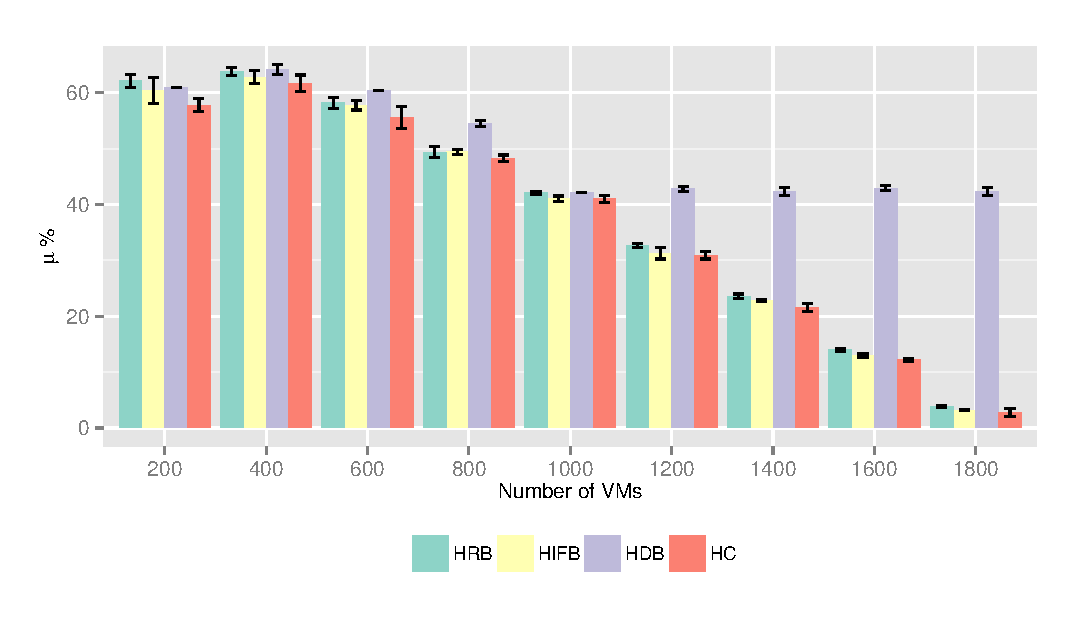
\includegraphics[width=1.0\linewidth]{figure28.eps}
	\captionof{figure}{Experiment 2: performance gain ($\mu$) over baseline execution with different number of resources for the LIGO workflow (number of tasks is 8000).}
	\label{fig:evaluation_resource_3}
\end{figure}

\paragraph{\textbf{Experiment 3}}
Figure~\ref{fig:evaluation_vc_cybershake} shows the performance gain $\mu$ for the Cybershake workflow over the baseline execution when using vertical clustering (VC) combined to our balancing methods. Vertical clustering does not {show }any improvement {for }the Cybershake workflow ($\mu$(\emph{VC-only}) $\approx 0.2\%$), because the workflow structure has no explicit pipeline{s }(see Figure~\ref{fig:evaluation_shape_cybershake}). Similarly, VC does not improve the SIPHT workflow due to the lack of pipelines {in }its structure (Figure~\ref{fig:evaluation_shape_sipht}). Thus, results for this workflow are omitted.

\begin{figure}[!htb]
	\centering
	\includegraphics[width=1.0\linewidth]{figure24.eps}
	\captionof{figure}{Experiment 3: performance gain ($\mu$) for the Cybershake workflow over baseline execution when using vertical clustering (VC).}
	\label{fig:evaluation_vc_cybershake}
\end{figure}

Figure~\ref{fig:evaluation_vc_montage} shows the performance gain $\mu$ for the Montage workflow. In this workflow, vertical clustering is often performed on the two pipelines (Figure~\ref{fig:evaluation_shape_montage}). These pipelines {have only a single task in each workflow level, }thereby no horizontal clustering is performed on the pipelines. As a result, whether performing vertical clustering prior or after horizontal clustering, the result is about the same. Since VC and horizontal clustering methods are independent {of }each other in this case, we {should still }do VC in combination with horizontal clustering to achieve further performance improvement. 

\begin{figure}[!htb]
	\centering
	\includegraphics[width=1.0\linewidth]{figure25.eps}
	\captionof{figure}{Experiment 3: performance gain ($\mu$) for the Montage workflow over baseline execution when using vertical clustering (VC).}
	\label{fig:evaluation_vc_montage}
\end{figure}

\begin{figure}[!htb]
	\centering
	\includegraphics[width=1.0\linewidth]{figure26.eps}
	\captionof{figure}{Experiment 3: performance gain ($\mu$) for the LIGO workflow over baseline execution when using vertical clustering (VC).}
	\label{fig:evaluation_vc_ligo}
\end{figure}


\begin{figure}[!htb]
	\centering
	\includegraphics[width=1.0\linewidth]{figure27.eps}
	\captionof{figure}{Experiment 3: performance gain ($\mu$) for the Epigenomics workflow over baseline execution when using vertical clustering (VC).}
	\label{fig:evaluation_vc_genome}
\end{figure}

The performance gain $\mu$ for the LIGO workflow is shown in Figure~\ref{fig:evaluation_vc_ligo}. Vertical clustering yields better performance gain when it is performed prior to horizontal clustering (\emph{VC-prior}). The LIGO workflow structure (Figure~\ref{fig:evaluation_shape_ligo}) has several pipelines that are primarily clustered vertically and thus system overheads (e.g. queuing and scheduling times) are reduced. Furthermore, the runtime variance (HRV) of the clustered pipelines increases, thus the balancing methods, in particular HRB, can further improve the runtime performance by evenly distributing task runtimes among clustered jobs. When vertical clustering is performed \emph{a posteriori}, pipelines are broken due to the {horizontal }merging of tasks between pipelines neutralizing vertical clustering improvements.

Similarly to the LIGO workflow, the performance gain $\mu$ values for the Epigenomics workflow (see Figure~\ref{fig:evaluation_vc_genome}) {is }better when VC is performed \emph{a priori}. This is due to several pipelines inherent to the workflow structure (Figure~\ref{fig:evaluation_shape_genome}). However, vertical clustering has poorer performance if it is performed prior to the HDB algorithm. The reason is the average task runtime of Epigenomics is much larger than {that of }other workflows as shown in Table.~\ref{tab:evaluation_workflows}. Therefore, \emph{VC-prior} generates very large clustered jobs vertically and makes it difficult for horizontal methods to improve further. 


\subsection{Compilation of the results}

The experimental results show strong relations between the proposed imbalance metrics and the performance improvement of the balancing methods. HRV indicates the potential performance improvement for HRB. The higher HRV, the more performance improvement HRB is likely to have. Similarly, for {the }workflows with symmetric structures (such as Epigenomics) where HIFV and HDV values are low, neither HIFB nor HDB performs well.

Based on the conclusions of the experimental evaluation, we applied machine learning techniques on the result data to build a decision tree that can be used to drive the development of {policy }engines {that can }select a {well performing }balancing method. Although our decision tree is tightly coupled to our results, it can be used by online systems that implement the {adaptive }MAPE-K loop~\cite{daSilva:2013:TFO:2534248.2534254,FerreiradaSilva-CCPE-2014,FerreiradaSilva-FGCS-2013}, which will adjust the tree according to the system behavior.

\begin{figure}[!htb]
	\centering
	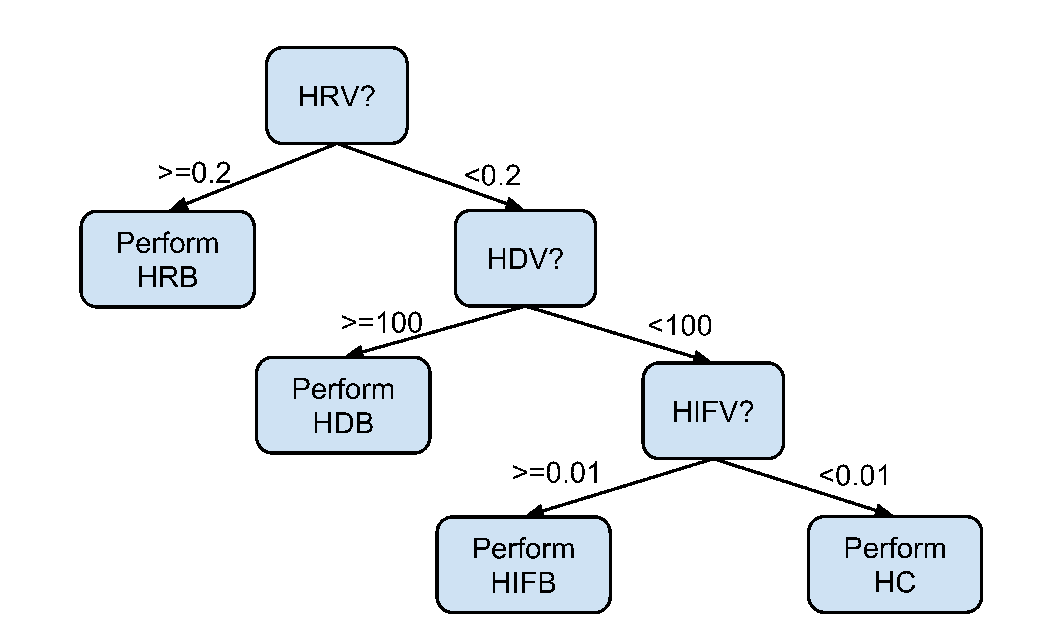
\includegraphics[width=1.0\linewidth]{figure29.eps}
	\captionof{figure}{Decision tree for selection of the appropriate balancing method.}
	\label{fig:decision_tree}
\end{figure}



%For the Epigenomics workflow as shown in Figure~\ref{fig:evaluation_vc_genome}, we observe similar phenomenon in HRB compared to the LIGO Inspiral workflow. As to the performance of HDB, VC-prior merges tasks at the second, third, fourth and fifth level together and thus HDB has less space to further improve the overall runtime. 

%Figure~\ref{fig:evaluation_wfsize} compares the performance gain of these algorithms by varying the workflow sizes (number of tasks in a workflow). By default, the LIGO Inspiral workflow in our paper has 800 tasks. With the decrease of workflow size, we can see that all of these methods perform worse. The reason is there is less resource contention with the decrease of workflow size and therefore task clustering does not perform well. The performance of HRB is more stable since the increase (or decrease) of workflow size has more significant impact on data transfer (roughly linear increase in runtime and square increase in data transfer). 

%The SIPHT workflow as shown in Figure~\ref{fig:evaluation_shape_sipht} does not have enough pipelines to perform vertical clustering and therefore we do not show its results of combining vertical clustering. 
 
%HIFB and HDB significantly increase the performance of the workflow execution. Both strategies capture the structural and runtime information, reducing data transfers between tasks, while HRB focuses on runtime distribution, which in this case is none. Figure~\ref{fig:imbalance_performance} (bottom) shows the performance of the balancing methods for the Epigenomics workflow. When increasing the average data size, only HDB demonstrates significantly improvement related to HC. Investigating the structure of the Epigenomics workflow (Figure~\ref{fig:imbalance_shape}-bottom), we can see that all tasks at the same horizontal level share the same IFs ($HIFV$ = 0), because each branch (surrounded by dash lines) happen to have the same amount of pipelines. Thus, HIFB has no performance improvement when compared to HC. However, for LIGO (Figure~\ref{fig:imbalance_shape}-top), $HIFV \neq 0$, thus HIFB improves the workflow runtime performance.  
%The intuition behind this difference between HDB and HIFB is that 
%HDB captures the strong connections between tasks (data dependencies) and HIFB captures the weak connections (similarity in terms of structure). In both workflows, $HDV$ is not zero thus HDB performs better than HC. 






\section{Conclusion and Future Work}

We presented three {task clustering methods that try to balance the workload across clusters and two vertical clustering variants. }We also defined three imbalance metrics to quantitatively measure workflow characteristics based on task runtime variation (HRV), task impact factor (HIFV), and task distance variance (HDV).

Three {sets of }experiment sets were conducted using traces from five real workflow applications. The first experiment aimed at measuring the performance gain over a baseline execution without clustering. In addition, we compared our balancing methods with three algorithms {described }in literature. Experimental results show that our methods yield {a }significant improvement over a baseline execution, and that they have acceptable performance when compared to {the }performance of the existing algorithms. The second experiment measured the influence of {the }average data size and {the }number of available resources on the performance gain. In particular, results show{ed }that our methods have different sensitivity to data- and computational-intensive workflows. Finally, the last experiment evaluated the {benefit }of performing horizontal and vertical clustering in the same workflow. Results show{ed }that vertical clustering can significantly improve pipeline-structured workflows, {but that }it is not suitable if the workflow has no explicit pipelines.

The simulation{-}based evaluation also show{ed }that the performance improvement of the proposed balancing algorithms (HRB, HDB and HIFB) is highly related to the metric values (HRV, HDV and HIFV) that we introduced. For example, a workflow with high HRV tends to have better performance improvement with HRB since HRB is used to balance the runtime variance. 

In the future, we plan to further analyze the imbalance metrics proposed. For instance, the values of {the }metrics presented in this paper are not normalized, and thus their values per level (HIFV, HDV, and HRV) are {at }different scales. Also, we plan to analyze more workflow applications, particularly the ones with asymmetric structures, to investigate the relationship between workflow structures and the metric values. 

Also, as shown in Figure~\ref{fig:evaluation_vc_genome}, \emph{VC-prior} can generate very large clustered jobs vertically and makes it difficult for horizontal methods to {further improve the workflow performance. }Therefore, we aim to develop imbalance metrics for \emph{VC-prior} to avoid generating large clustered jobs, i.e., based on the accumulated runtime of tasks in a pipeline. 

As shown in our experiment{al }results, the combination of our balancing methods with vertical clustering {has }different sensitivity to workflows with {different }graph structures and runtime distribution. Therefore, a possible future work is the development of a portfolio clustering {algorithm, }which chooses multiple clustering algorithms, and dynamically selects {the }most suitable one according to the dynamic load.

%In this manuscript, we demonstrate the performance gain of combining horizontal clustering methods and vertical clustering. We plan to combine multiple algorithms together instead of just two. We will develop a policy engine that iteratively chooses one algorithm from all of the balancing methods based on the imbalance metrics until the performance gain converges. 

%Finally, we aim at applying our metrics to other workflow study areas, such as workflow scheduling where heuristics would either look into the characteristics of the task when it is ready to schedule (local scheduling), or examine the entire workflow (global optimization algorithms). In this work, the impact factor metric only uses a family of tasks that are tightly related or similar to each other. This method represents a new approach to solve the existing problems. 

\section*{Acknowledgements}
\footnotesize
This work was funded by NSF IIS-0905032 and NSF FutureGrid 0910812 awards. We thank Gideon Juve, Karan Vahi, Rajiv Mayani, and Mats Rynge for their valuable help. 




%% References with bibTeX database:

\bibliographystyle{elsarticle-num}
\begin{thebibliography}{10}
\expandafter\ifx\csname url\endcsname\relax
  \def\url#1{\texttt{#1}}\fi
\expandafter\ifx\csname urlprefix\endcsname\relax\def\urlprefix{URL }\fi
\expandafter\ifx\csname href\endcsname\relax
  \def\href#1#2{#2} \def\path#1{#1}\fi

\bibitem{daSilva:2013:TFO:2534248.2534254}
R.~Ferreira~da Silva, G.~Juve, E.~Deelman, T.~Glatard, F.~Desprez, D.~Thain,
  B.~Tovar, M.~Livny, Toward fine-grained online task characteristics
  estimation in scientific workflows, in: Proceedings of the 8th Workshop on
  Workflows in Support of Large-Scale Science, WORKS '13, ACM, 2013, pp.
  58--67.
\bibitem{rizos2008}
L.~Canon, E.~Jeannot, R.~Sakellariou and W.~Zheng, Comparative Evaluation Of The Robustness Of DAG Scheduling Heuristics, Grid Computing, 2008, pp.~73-84


\bibitem{Juve2013}
G.~Juve, A.~Chervenak, E.~Deelman, S.~Bharathi, G.~Mehta, K.~Vahi,
  Characterizing and profiling scientific workflows, Vol.~29, 2013, pp. 682 --
  692, special Section: Recent Developments in High Performance Computing and
  Security.


\bibitem{Chen2011}
W.~Chen, E.~Deelman, Workflow overhead analysis and optimizations, in:
  Proceedings of the 6th workshop on Workflows in support of large-scale
  science, WORKS '11, 2011, pp. 11--20.

\bibitem{Muthuvelu:2005:DJG:1082290.1082297}
N.~Muthuvelu, J.~Liu, N.~L. Soe, S.~Venugopal, A.~Sulistio, R.~Buyya, A dynamic
  job grouping-based scheduling for deploying applications with fine-grained
  tasks on global grids, in: Proceedings of the 2005 Australasian workshop on
  Grid computing and e-research - Volume 44, 2005, pp. 41--48.

\bibitem{4493929}
N.~Muthuvelu, I.~Chai, C.~Eswaran, An adaptive and parameterized job grouping
  algorithm for scheduling grid jobs, in: Advanced Communication Technology,
  2008. ICACT 2008. 10th International Conference on, Vol.~2, 2008, pp. 975
  --980.

\bibitem{Muthuvelu2010}
N.~Muthuvelu, I.~Chai, E.~Chikkannan, R.~Buyya, On-line task granularity
  adaptation for dynamic grid applications, in: Algorithms and Architectures
  for Parallel Processing, Vol. 6081 of Lecture Notes in Computer Science,
  2010, pp. 266--277.

\bibitem{Muthuvelu2013170}
N.~Muthuvelu, C.~Vecchiolab, I.~Chaia, E.~Chikkannana, R.~Buyyab, Task
  granularity policies for deploying bag-of-task applications on global grids,
  Future Generation Computer Systems 29~(1) (2012) 170 -- 181.

\bibitem{keat-2006}
W.~K. Ng, T.~Ang, T.~Ling, C.~Liew, Scheduling framework for bandwidth-aware
  job grouping-based scheduling in grid computing, Malaysian Journal of
  Computer Science 19~(2) (2006) 117--126.

\bibitem{ang-2009}
T.~Ang, W.~Ng, T.~Ling, L.~Por, C.~Lieu, A bandwidth-aware job grouping-based
  scheduling on grid environment, Information Technology Journal 8 (2009)
  372--377.

\bibitem{Liu2009}
Q.~Liu, Y.~Liao, Grouping-based fine-grained job scheduling in grid computing,
  in: First International Workshop on Education Technology and Computer
  Science, Vol.~1, 2009, pp. 556 --559.

\bibitem{Singh:2008:WTC:1341811.1341822}
G.~Singh, M.-H. Su, K.~Vahi, E.~Deelman, B.~Berriman, J.~Good, D.~S. Katz,
  G.~Mehta, Workflow task clustering for best effort systems with pegasus, in:
  15th {ACM} Mardi Gras Conference, 2008, pp. 9:1--9:8.

\bibitem{Ferreira-granularity-2013}
R.~Ferreira~da Silva, T.~Glatard, F.~Desprez, On-line, non-clairvoyant
  optimization of workflow activity granularity on grids, in: F.~Wolf, B.~Mohr,
  D.~Mey (Eds.), Euro-Par 2013 Parallel Processing, Vol. 8097 of Lecture Notes
  in Computer Science, Springer Berlin Heidelberg, 2013, pp. 255--266.


\bibitem{Chen2013}
W.~Chen, E.~Deelman, R.~Sakellariou, Imbalance optimization in scientific
  workflows, in: Proceedings of the 27th international ACM conference on
  International conference on supercomputing, ICS '13, 2013, pp. 461--462.

\bibitem{Lifflander}
J.~Lifflander, S.~Krishnamoorthy, L.~V. Kale, Work stealing and
  persistence-based load balancers for iterative overdecomposed applications,
  in: Proceedings of the 21st international symposium on High-Performance
  Parallel and Distributed Computing, HPDC '12, 2012, pp. 137--148.

\bibitem{6217508}
W.~Chen, E.~Deelman, Integration of workflow partitioning and resource
  provisioning, in: Cluster, Cloud and Grid Computing (CCGrid), 2012 12th
  IEEE/ACM International Symposium on, 2012, pp. 764--768.

\bibitem{6683907}
W.~Chen, R.~Ferreira~da Silva, E.~Deelman, R.~Sakellariou, Balanced task
  clustering in scientific workflows, in: eScience (eScience), 2013 IEEE 9th
  International Conference on, 2013, pp. 188--195.

\bibitem{Ostberg2011}
P.-O. OÃàstberg, E.~Elmroth, Mediation of service overhead in service-oriented
  grid architectures, in: Grid Computing (GRID), 2011 12th IEEE/ACM
  International Conference on, 2011, pp. 9--18.

\bibitem{Prodan2008}
R.~Prodan, T.~Fabringer, Overhead analysis of scientific workflows in grid
  environments, in: IEEE Transactions in Parallel and Distributed System,
  Vol.~19, 2008.

\bibitem{Stratan2008}
C.~Stratan, A.~Iosup, D.~H. Epema, A performance study of grid workflow
  engines, in: Grid Computing, 2008 9th IEEE/ACM International Conference on,
  IEEE, 2008, pp. 25--32.

\bibitem{FerreiradaSilva-CCPE-2014}
R.~Ferreira~da Silva, T.~Glatard, F.~Desprez, Controlling fairness and task
  granularity in distributed, online, non-clairvoyant workflow executions,
  Concurrency and Computation: Practice and Experience (2014) in press.

\bibitem{Zheng}
G.~Zheng, A.~Bhatel{\'e}, E.~Meneses, L.~V. Kal{\'e}, Periodic hierarchical
  load balancing for large supercomputers, Int. J. High Perform. Comput. Appl.
  25~(4) (2011) 371--385.

\bibitem{22559942}
	M.~Abouelhoda, S.~Issa, and M.~Ghanem, Tavaxy: Integrating Taverna and Galaxy workflows with cloud computing support, BMC Bioinformatics,
	Vol.~13, 2012, pp. 77.
	
	
\bibitem{goecks2010galaxy}
 J.~Goecks, A.~Nekrutenko and et.al., Galaxy: a comprehensive approach for supporting accessible, reproducible, and transparent computational research in the life sciences, 
Genome Biol,  vol.~11, 2010.

\bibitem{deelman2014pegasus}
E.~Deelman, K.~Vahi, G.~Juve, M.~Rynge, S.~Callaghan, P.~Maechling, R.~Mayani, W.~Chen, R.~Ferreira~da Silva, M.~Livny, and K.~Wenger, Pegasus, a Workflow Management System for Science Automation, submitted to Future Generation Computer Systems, 2014, 
% Pegasus
bibitem{Deelman:2005:PFM:1239649.1239653}
E.~Deelman, and et. al., Pegasus: A Framework for Mapping Complex Scientific Workflows Onto Distributed Systems, Sci. Program., vol.~13, 2005, pp. 219-237.




\bibitem{Yu2005}
J.~Yu, R.~Buyya, A taxonomy of workflow management systems for grid computing,
  Journal of Grid Computing 3.

\bibitem{Liu2008}
X.~Liu, J.~Chen, K.~Liu, Y.~Yang, Forecasting duration intervals of scientific
  workflow activities based on time-series patterns, in: eScience, 2008.
  eScience '08. IEEE Fourth International Conference on, 2008, pp. 23--30.

\bibitem{Deelman2004}
E.~Deelman, J.~Blythe, Y.~Gil, C.~Kesselman, G.~Mehta, S.~Patil, M.~Su,
  K.~Vahi, M.~Livny, Pegasus: Mapping scientific workflows onto the grid, in:
  Across Grid Conference, 2004.

\bibitem{Ali2004}
S.~Ali, A.~Maciejewski, H.~Siegel, J.-K. Kim, Measuring the robustness of a
  resource allocation, Parallel and Distributed Systems, IEEE Transactions on
  15~(7) (2004) 630--641.

\bibitem{Tolosana2011}
R.~Tolosana-Calasanz, M.~Lackovic, O.~F~Rana, J.~{\'A}. Ba{\~n}ares, D.~Talia,
  Characterizing quality of resilience in scientific workflows, in: Proceedings
  of the 6th workshop on Workflows in support of large-scale science, ACM,
  2011, pp. 117--126.

\bibitem{Ma:2014:GDB:2560969.2561388}
Y.~Ma, X.~Zhang, K.~Lu, A graph distance based metric for data oriented
  workflow retrieval with variable time constraints, Expert Syst. Appl. 41~(4)
  (2014) 1377--1388.

\bibitem{Deelman:2005:PFM:1239649.1239653}
E.~Deelman, G.~Singh, M.-H. Su, J.~Blythe, Y.~Gil, C.~Kesselman, G.~Mehta,
  K.~Vahi, G.~B. Berriman, J.~Good, A.~Laity, J.~C. Jacob, D.~S. Katz, Pegasus:
  A framework for mapping complex scientific workflows onto distributed
  systems, Sci. Program. 13~(3) (2005) 219--237.

\bibitem{Fahringer:2005:ATS:1064323.1064331}
T.~Fahringer, A.~Jugravu, S.~Pllana, R.~Prodan, C.~Seragiotto, Jr., H.-L.
  Truong, Askalon: a tool set for cluster and grid computing: Research
  articles, Concurr. Comput. : Pract. Exper. 17~(2-4) (2005) 143--169.

\bibitem{Oinn:2006:TLC:1148437.1148448}
T.~Oinn, M.~Greenwood, M.~Addis, M.~N. Alpdemir, J.~Ferris, K.~Glover,
  C.~Goble, A.~Goderis, D.~Hull, D.~Marvin, P.~Li, P.~Lord, M.~R. Pocock,
  M.~Senger, R.~Stevens, A.~Wipat, C.~Wroe, Taverna: lessons in creating a
  workflow environment for the life sciences: Research articles, Concurr.
  Comput. : Pract. Exper. 18~(10) (2006) 1067--1100.

\bibitem{LIGO}
D.~Brown, P.~Brady, A.~Dietz, J.~Cao, B.~Johnson, J.~McNabb, A case study on
  the use of workflow technologies for scientific analysis: Gravitational wave
  data analysis, in: I.~Taylor, E.~Deelman, D.~Gannon, M.~Shields (Eds.),
  Workflows for e-Science, Springer London, 2007, pp. 39--59.


\bibitem{Berriman2004}
G.~B. Berriman, E.~Deelman, J.~C. Good, J.~C. Jacob, D.~S. Katz, C.~Kesselman,
  A.~C. Laity, T.~A. Prince, G.~Singh, M.~Su, Montage: a grid-enabled engine
  for delivering custom science-grade mosaics on demand, in: {SPIE Conference
  on Astronomical Telescopes and Instrumentation}, Vol. 5493, 2004, pp.
  221--232.


\bibitem{Graves2010}
R.~Graves, T.~Jordan, S.~Callaghan, E.~Deelman, E.~Field, G.~Juve,
  C.~Kesselman, P.~Maechling, G.~Mehta, K.~Milner, D.~Okaya, P.~Small, K.~Vahi,
  {CyberShake: A Physics-Based Seismic Hazard Model for Southern California},
  Pure and Applied Geophysics 168~(3-4) (2011) 367--381.


\bibitem{Epigenome}
{USC Epigenome Center}, \url{http://epigenome.usc.edu}.

\bibitem{SIPHT}
{SIPHT}, \url{http://pegasus.isi.edu/applications/sipht}.

\bibitem{Chen2012a}
W.~Chen, E.~Deelman, Workflowsim: A toolkit for simulating scientific workflows
  in distributed environments, in: E-Science (e-Science), 2012 IEEE 8th
  International Conference on, 2012, pp. 1--8.


\bibitem{Calheiros2011}
R.~N. Calheiros, R.~Ranjan, A.~Beloglazov, C.~A.~F. De~Rose, R.~Buyya,
  {CloudSim:} a toolkit for modeling and simulation of cloud computing
  environments and evaluation of resource provisioning algorithms, Software:
  Practice and Experience 41~(1) (2011) 23--50.

\bibitem{Chen2012}
W.~Chen, E.~Deelman, Fault tolerant clustering in scientific workflows, in:
  Services (SERVICES), 2012 IEEE Eighth World Congress on, 2012, pp. 9--16.

\bibitem{jrad2013broker}
F.~Jrad, J.~Tao, A.~Streit, A broker-based framework for multi-cloud workflows,
  in: Proceedings of the 2013 international workshop on Multi-cloud
  applications and federated clouds, ACM, 2013, pp. 61--68.

\bibitem{AmazonAWS}
{Amazon.com, Inc.}, \href{http://aws.amazon.com}{{Amazon Web Services}},
  \url{http://aws.amazon.com}.
\newline\urlprefix\url{http://aws.amazon.com}

\bibitem{FutureGrid}
{FutureGrid}, \url{http://futuregrid.org/}.

\bibitem{Juve09scientificworkflow}
G.~Juve, E.~Deelman, K.~Vahi, G.~Mehta, B.~Berriman, Scientific workflow
  applications on amazon ec2, in: In Cloud Computing Workshop in Conjunction
  with e-Science, IEEE, 2009.

\bibitem{FerreiradaSilva-eScience-2014}
R.~Ferreira~da Silva, W.~Chen, G.~Juve, K.~Vahi, E.~Deelman, Community
  resources for enabling and evaluating research on scientific workflows, in:
  10th IEEE International Conference on e-Science, eScience'14, 2014, p. to
  appear.

\bibitem{FerreiradaSilva-FGCS-2013}
R.~Ferreira~da Silva, T.~Glatard, F.~Desprez, Self-healing of workflow activity
  incidents on distributed computing infrastructures, Future Generation
  Computer Systems 29~(8) (2013) 2284--2294.

\end{thebibliography}


\end{document}